% Conference version of paper 1 (17 Nov 2026, laptop strengthening item 3): the break-even rule, its tests and its
% hardware check. Same metric files as main.tex; every number is a generated macro. Build: bash build_conf.sh
\documentclass[conference,10pt]{IEEEtran}
\usepackage{amsmath,amssymb,amsthm}
\usepackage{booktabs}
\usepackage{graphicx}
\usepackage{cite}
\usepackage{url}
\usepackage[hidelinks]{hyperref}
\graphicspath{{figures/}}

% Generated by evaluation/make_tables.py -- do not edit.
% Generated by evaluation/make_tables.py from experiments/results -- do not edit.
\newcommand{\NumValImages}{5,000}
\newcommand{\NBootAccuracy}{300}
\newcommand{\NBootCodec}{200}
\newcommand{\BaselineMAP}{44.4}
\newcommand{\BaselineMAPfifty}{61.1}
\newcommand{\TotalGFLOPs}{28.8}
\newcommand{\TotalParamsM}{11.17}
\newcommand{\MaxAbsDeltaINT}{0.04}
\newcommand{\MaxAbsDeltaFPsixteen}{0.003}
\newcommand{\NumSignificantINT}{0}
\newcommand{\SignificantINTCuts}{none}
\newcommand{\SignificanceSentence}{no cut shows a statistically detectable change (every 95\% interval includes zero)}
\newcommand{\DeltaINTKTwo}{$-$0.01 [$-$0.03, +0.02]}
\newcommand{\DeltaINTKFour}{$-$0.01 [$-$0.06, +0.03]}
\newcommand{\DeltaINTKFive}{0.00 [$-$0.02, +0.03]}
\newcommand{\DeltaINTKSeven}{$-$0.04 [$-$0.09, 0.00]}
\newcommand{\DeltaINTKNine}{$-$0.03 [$-$0.06, 0.00]}
\newcommand{\DeltaINTKTwelve}{$-$0.01 [$-$0.04, +0.02]}
\newcommand{\DeltaINTKFifteen}{0.00 [$-$0.03, +0.03]}
\newcommand{\DeltaINTKEighteen}{0.00 [$-$0.03, +0.03]}
\newcommand{\DeltaClip}{$-$0.14 [$-$0.23, $-$0.02]}
\newcommand{\DeltaPerChannel}{0.00 [$-$0.02, +0.01]}
\newcommand{\DeltaUINT}{$-$0.01 [$-$0.03, +0.01]}
\newcommand{\RawImageKiB}{1,200.0}
\newcommand{\PayloadINTKTwo}{1,600.0}
\newcommand{\PayloadZstdKTwo}{642.2}
\newcommand{\FlopPctKTwo}{9.3}
\newcommand{\PayloadINTKFour}{800.0}
\newcommand{\PayloadZstdKFour}{310.7}
\newcommand{\FlopPctKFour}{21.4}
\newcommand{\PayloadINTKFive}{1,200.0}
\newcommand{\PayloadZstdKFive}{473.4}
\newcommand{\FlopPctKFive}{24.7}
\newcommand{\PayloadINTKSeven}{1,400.1}
\newcommand{\PayloadZstdKSeven}{555.9}
\newcommand{\FlopPctKSeven}{36.7}
\newcommand{\PayloadINTKNine}{1,400.1}
\newcommand{\PayloadZstdKNine}{541.6}
\newcommand{\FlopPctKNine}{43.7}
\newcommand{\PayloadINTKTwelve}{1,400.1}
\newcommand{\PayloadZstdKTwelve}{559.3}
\newcommand{\FlopPctKTwelve}{50.2}
\newcommand{\PayloadINTKFifteen}{1,400.1}
\newcommand{\PayloadZstdKFifteen}{614.5}
\newcommand{\FlopPctKFifteen}{56.9}
\newcommand{\PayloadINTKEighteen}{1,400.1}
\newcommand{\PayloadZstdKEighteen}{594.6}
\newcommand{\FlopPctKEighteen}{64.0}
\newcommand{\LiveElemsKFiveM}{1.2}
\newcommand{\LiveElemsKSevenM}{1.4}
\newcommand{\ZstdRatioMin}{2.3}
\newcommand{\ZstdRatioMax}{2.6}
\newcommand{\MinSplitKiB}{310.7}
\newcommand{\MinSplitCut}{$k_{4}$}
\newcommand{\JPEGKiBQFifty}{36.5}
\newcommand{\JPEGDeltaQFifty}{$-$3.48 [$-$3.80, $-$3.11]}
\newcommand{\JPEGLossQFifty}{3.48}
\newcommand{\JPEGEncMsQFifty}{0.79}
\newcommand{\JPEGKiBQSeventyFive}{54.0}
\newcommand{\JPEGDeltaQSeventyFive}{$-$1.29 [$-$1.51, $-$1.04]}
\newcommand{\JPEGLossQSeventyFive}{1.29}
\newcommand{\JPEGEncMsQSeventyFive}{0.87}
\newcommand{\JPEGKiBQNinety}{91.0}
\newcommand{\JPEGDeltaQNinety}{$-$0.33 [$-$0.47, $-$0.20]}
\newcommand{\JPEGLossQNinety}{0.33}
\newcommand{\JPEGEncMsQNinety}{1.03}
\newcommand{\JPEGKiBQNinetyFive}{130.9}
\newcommand{\JPEGDeltaQNinetyFive}{$-$0.21 [$-$0.30, $-$0.10]}
\newcommand{\JPEGLossQNinetyFive}{0.21}
\newcommand{\JPEGEncMsQNinetyFive}{1.10}
\newcommand{\RatioKFourOverJPEG}{8.8}
\newcommand{\RatioMinSplitOverJPEG}{3.4}
\newcommand{\RatioMinSplitOverJPEGQNinetyFive}{2.4}
\newcommand{\RatioKFourOverJPEGQNinetyFive}{6.1}
\newcommand{\HTwoSixFourBestKiB}{115.8}
\newcommand{\HTwoSixFourBestCRF}{18}
\newcommand{\HostGPU}{NVIDIA GeForce RTX 4050 Laptop GPU}
\newcommand{\TimingImages}{200}
\newcommand{\HostFullMs}{11.93}
\newcommand{\HostEdgeKFourMs}{1.81}
\newcommand{\HostQuantKFourMs}{0.45}
\newcommand{\HostSerKFourMs}{0.60}
\newcommand{\HostCloudKFourMs}{5.42}
\newcommand{\HostZstdSerKFourMs}{2.03}
\newcommand{\SQNRINT}{28.3}
\newcommand{\SQNRPerChannel}{35.2}
\newcommand{\SQNRFPsixteen}{73.6}
\newcommand{\BoundRatioMax}{1.000000}
\newcommand{\HoverW}{109.9}
\newcommand{\AtwoASpacingM}{50}
\newcommand{\AtwoASpacingMbps}{59.7}
\newcommand{\AtwoARangeM}{840}
\newcommand{\AtwoAShadowDb}{3.0}
\newcommand{\AtwoAMacEff}{0.65}
\newcommand{\AtwoAPerThreshold}{10}
\newcommand{\AtwoAPerSlope}{2}
\newcommand{\RelayThresholdMbps}{5}
\newcommand{\RelayNeighbourMinMbps}{15}
\newcommand{\PolicyDelayMs}{20}
\newcommand{\PolicyTauMs}{200}
\newcommand{\PolicyHysteresisPct}{5}
\newcommand{\PolicySigmaFloor}{0.1}
\newcommand{\PolicyEnergyWeight}{0.05}
\newcommand{\AvionicsW}{15.0}
\newcommand{\BatteryWh}{55.5}
\newcommand{\PComputeW}{10.0}
\newcommand{\PIdleW}{2.0}
\newcommand{\PTxW}{3.8}
\newcommand{\PRxW}{1.2}
\newcommand{\ShannonAlpha}{0.4}
\newcommand{\ShannonSEMax}{2}
\newcommand{\ShannonSINRMin}{-10}
\newcommand{\TraceGoodMeanMbps}{63.0}
\newcommand{\TraceGoodPFiveMbps}{39.2}
\newcommand{\TraceGoodOutagePct}{0.0}
\newcommand{\TraceModerateMeanMbps}{24.6}
\newcommand{\TraceModeratePFiveMbps}{8.5}
\newcommand{\TraceModerateOutagePct}{0.0}
\newcommand{\TraceBlackoutMeanMbps}{30.1}
\newcommand{\TraceBlackoutPFiveMbps}{0.0}
\newcommand{\TraceBlackoutOutagePct}{5.3}
\newcommand{\TraceFadingMeanMbps}{21.1}
\newcommand{\TraceFadingPFiveMbps}{3.8}
\newcommand{\TraceFadingOutagePct}{0.4}
\newcommand{\NumSeeds}{5}
\newcommand{\SweepTfullMinMs}{40}
\newcommand{\SweepTfullMaxMs}{360}
\newcommand{\SysGoodOnboardFPS}{5.0}
\newcommand{\SysGoodOnboardPNinetyFive}{180}
\newcommand{\SysGoodOnboardPowerW}{10.4}
\newcommand{\SysGoodSplitKFourFPS}{10.6}
\newcommand{\SysGoodSplitKFourPNinetyFive}{244}
\newcommand{\SysGoodSplitKFourPowerW}{12.3}
\newcommand{\SysGoodSplitKFourZstdFPS}{10.0}
\newcommand{\SysGoodSplitKFourZstdPNinetyFive}{155}
\newcommand{\SysGoodSplitKFourZstdPowerW}{10.4}
\newcommand{\SysGoodSplitKNineFPS}{0.0}
\newcommand{\SysGoodSplitKNinePNinetyFive}{322}
\newcommand{\SysGoodSplitKNinePowerW}{12.9}
\newcommand{\SysGoodJPEGFPS}{30.0}
\newcommand{\SysGoodJPEGPNinetyFive}{60}
\newcommand{\SysGoodJPEGPowerW}{7.8}
\newcommand{\SysGoodAdaptiveSplitFPS}{10.0}
\newcommand{\SysGoodAdaptiveSplitPNinetyFive}{161}
\newcommand{\SysGoodAdaptiveSplitPowerW}{10.4}
\newcommand{\SysGoodAdaptiveAllFPS}{30.0}
\newcommand{\SysGoodAdaptiveAllPNinetyFive}{65}
\newcommand{\SysGoodAdaptiveAllPowerW}{8.1}
\newcommand{\SysModerateOnboardFPS}{5.0}
\newcommand{\SysModerateOnboardPNinetyFive}{180}
\newcommand{\SysModerateOnboardPowerW}{10.4}
\newcommand{\SysModerateSplitKFourFPS}{0.4}
\newcommand{\SysModerateSplitKFourPNinetyFive}{337}
\newcommand{\SysModerateSplitKFourPowerW}{12.3}
\newcommand{\SysModerateSplitKFourZstdFPS}{6.5}
\newcommand{\SysModerateSplitKFourZstdPNinetyFive}{325}
\newcommand{\SysModerateSplitKFourZstdPowerW}{11.8}
\newcommand{\SysModerateSplitKNineFPS}{0.0}
\newcommand{\SysModerateSplitKNinePNinetyFive}{nan}
\newcommand{\SysModerateSplitKNinePowerW}{12.9}
\newcommand{\SysModerateJPEGFPS}{25.9}
\newcommand{\SysModerateJPEGPNinetyFive}{134}
\newcommand{\SysModerateJPEGPowerW}{9.2}
\newcommand{\SysModerateAdaptiveSplitFPS}{7.4}
\newcommand{\SysModerateAdaptiveSplitPNinetyFive}{309}
\newcommand{\SysModerateAdaptiveSplitPowerW}{11.4}
\newcommand{\SysModerateAdaptiveAllFPS}{29.7}
\newcommand{\SysModerateAdaptiveAllPNinetyFive}{95}
\newcommand{\SysModerateAdaptiveAllPowerW}{7.9}
\newcommand{\SysBlackoutOnboardFPS}{5.0}
\newcommand{\SysBlackoutOnboardPNinetyFive}{180}
\newcommand{\SysBlackoutOnboardPowerW}{10.4}
\newcommand{\SysBlackoutSplitKFourFPS}{1.3}
\newcommand{\SysBlackoutSplitKFourPNinetyFive}{330}
\newcommand{\SysBlackoutSplitKFourPowerW}{12.3}
\newcommand{\SysBlackoutSplitKFourZstdFPS}{8.9}
\newcommand{\SysBlackoutSplitKFourZstdPNinetyFive}{285}
\newcommand{\SysBlackoutSplitKFourZstdPowerW}{11.6}
\newcommand{\SysBlackoutSplitKNineFPS}{0.0}
\newcommand{\SysBlackoutSplitKNinePNinetyFive}{nan}
\newcommand{\SysBlackoutSplitKNinePowerW}{12.9}
\newcommand{\SysBlackoutJPEGFPS}{27.9}
\newcommand{\SysBlackoutJPEGPNinetyFive}{99}
\newcommand{\SysBlackoutJPEGPowerW}{8.9}
\newcommand{\SysBlackoutAdaptiveSplitFPS}{9.2}
\newcommand{\SysBlackoutAdaptiveSplitPNinetyFive}{279}
\newcommand{\SysBlackoutAdaptiveSplitPowerW}{11.5}
\newcommand{\SysBlackoutAdaptiveAllFPS}{28.5}
\newcommand{\SysBlackoutAdaptiveAllPNinetyFive}{77}
\newcommand{\SysBlackoutAdaptiveAllPowerW}{7.9}
\newcommand{\SysFadingOnboardFPS}{5.0}
\newcommand{\SysFadingOnboardPNinetyFive}{180}
\newcommand{\SysFadingOnboardPowerW}{10.4}
\newcommand{\SysFadingSplitKFourFPS}{0.4}
\newcommand{\SysFadingSplitKFourPNinetyFive}{336}
\newcommand{\SysFadingSplitKFourPowerW}{12.3}
\newcommand{\SysFadingSplitKFourZstdFPS}{4.9}
\newcommand{\SysFadingSplitKFourZstdPNinetyFive}{327}
\newcommand{\SysFadingSplitKFourZstdPowerW}{11.8}
\newcommand{\SysFadingSplitKNineFPS}{0.0}
\newcommand{\SysFadingSplitKNinePNinetyFive}{nan}
\newcommand{\SysFadingSplitKNinePowerW}{12.9}
\newcommand{\SysFadingJPEGFPS}{21.6}
\newcommand{\SysFadingJPEGPNinetyFive}{163}
\newcommand{\SysFadingJPEGPowerW}{9.3}
\newcommand{\SysFadingAdaptiveSplitFPS}{6.4}
\newcommand{\SysFadingAdaptiveSplitPNinetyFive}{298}
\newcommand{\SysFadingAdaptiveSplitPowerW}{11.1}
\newcommand{\SysFadingAdaptiveAllFPS}{27.2}
\newcommand{\SysFadingAdaptiveAllPNinetyFive}{122}
\newcommand{\SysFadingAdaptiveAllPowerW}{8.1}
\newcommand{\EnduranceMin}{24.2}
\newcommand{\EnduranceMax}{25.1}
\newcommand{\PerceptionPowerMinW}{7.8}
\newcommand{\PerceptionPowerMaxW}{12.9}
\newcommand{\NumCells}{16}
\newcommand{\JPEGWins}{16}
\newcommand{\SplitWins}{0}
\newcommand{\OnboardWins}{0}
\newcommand{\AdaptiveSplitGainMin}{0.94}
\newcommand{\AdaptiveSplitGainMax}{1.28}
\newcommand{\AdaptiveAllGainMin}{1.00}
\newcommand{\AdaptiveAllGainMax}{1.26}
\newcommand{\SplitBeatsOnboardCells}{10}
\newcommand{\JPEGOverBestSplitMin}{1.1}
\newcommand{\BwReqJPEGTForty}{2.8}
\newcommand{\BwReqKFourTForty}{25.5}
\newcommand{\BwReqKFourZstdTForty}{10.1}
\newcommand{\BwReqJPEGTOneEighty}{3.0}
\newcommand{\BwReqKFourTOneEighty}{30.5}
\newcommand{\BwReqKFourZstdTOneEighty}{13.3}
\newcommand{\SwarmMaxN}{20}
\newcommand{\CellCapacityMbps}{100}
\newcommand{\SwarmModerateAdaptiveSplitOne}{7.4}
\newcommand{\SwarmModerateAdaptiveSplitMax}{4.3}
\newcommand{\SwarmModerateAdaptiveSplitMaxRelay}{4.3}
\newcommand{\SwarmModerateAdaptiveSplitRelayedOnTime}{0}
\newcommand{\SwarmModerateAdaptiveSplitRelayed}{0}
\newcommand{\SwarmModerateAdaptiveAllOne}{29.7}
\newcommand{\SwarmModerateAdaptiveAllMax}{16.6}
\newcommand{\SwarmModerateAdaptiveAllMaxRelay}{16.6}
\newcommand{\SwarmModerateAdaptiveAllRelayedOnTime}{189}
\newcommand{\SwarmModerateAdaptiveAllRelayed}{193}
\newcommand{\SwarmModerateSplitKFourZstdOne}{6.5}
\newcommand{\SwarmModerateSplitKFourZstdMax}{0.0}
\newcommand{\SwarmModerateSplitKFourZstdMaxRelay}{0.0}
\newcommand{\SwarmModerateSplitKFourZstdRelayedOnTime}{0}
\newcommand{\SwarmModerateSplitKFourZstdRelayed}{66}
\newcommand{\SwarmBlackoutAdaptiveSplitOne}{9.2}
\newcommand{\SwarmBlackoutAdaptiveSplitMax}{4.1}
\newcommand{\SwarmBlackoutAdaptiveSplitMaxRelay}{4.1}
\newcommand{\SwarmBlackoutAdaptiveSplitRelayedOnTime}{0}
\newcommand{\SwarmBlackoutAdaptiveSplitRelayed}{0}
\newcommand{\SwarmBlackoutAdaptiveAllOne}{28.5}
\newcommand{\SwarmBlackoutAdaptiveAllMax}{16.7}
\newcommand{\SwarmBlackoutAdaptiveAllMaxRelay}{16.7}
\newcommand{\SwarmBlackoutAdaptiveAllRelayedOnTime}{83}
\newcommand{\SwarmBlackoutAdaptiveAllRelayed}{136}
\newcommand{\SwarmBlackoutSplitKFourZstdOne}{8.9}
\newcommand{\SwarmBlackoutSplitKFourZstdMax}{0.0}
\newcommand{\SwarmBlackoutSplitKFourZstdMaxRelay}{0.0}
\newcommand{\SwarmBlackoutSplitKFourZstdRelayedOnTime}{0}
\newcommand{\SwarmBlackoutSplitKFourZstdRelayed}{1,205}
\newcommand{\RelaySplitOnTime}{36}
\newcommand{\RelaySplitTotal}{2,254}
\newcommand{\RelayAdaptiveAllOnTime}{463}
\newcommand{\RelayAdaptiveAllTotal}{540}
\newcommand{\RelayMaxGain}{0.05}
\newcommand{\RelayMaxLoss}{0.3}
\newcommand{\SwarmAdaptiveSplitMaxNWorst}{4.1}
\newcommand{\SwarmOnboardFPS}{5.0}

% Generated by evaluation/make_generalization.py from experiments/results -- do not edit.
\newcommand{\GenDominanceTmin}{13}
\newcommand{\GenPhiRhoKFour}{0.43}
\newcommand{\GenRhoJpegMax}{0.09}
\newcommand{\GenAccBoundNinetyPct}{0.7}
\newcommand{\GenAccBoundNinetyFivePct}{0.4}
\newcommand{\GenBitsTwoKiB}{0.5}
\newcommand{\GenBitsTwoDelta}{$-$44.38 [$-$45.81, $-$43.79]}
\newcommand{\GenBitsThreeKiB}{23.0}
\newcommand{\GenBitsThreeDelta}{$-$22.10 [$-$22.93, $-$21.42]}
\newcommand{\GenBitsFourKiB}{54.4}
\newcommand{\GenBitsFourDelta}{$-$8.07 [$-$8.57, $-$7.60]}
\newcommand{\GenBitsFiveKiB}{138.6}
\newcommand{\GenBitsFiveDelta}{$-$3.51 [$-$3.85, $-$3.19]}
\newcommand{\GenBitsSixKiB}{181.5}
\newcommand{\GenBitsSixDelta}{$-$0.21 [$-$0.33, $-$0.11]}
\newcommand{\GenBitsSevenKiB}{241.2}
\newcommand{\GenBitsSevenDelta}{$-$0.03 [$-$0.08, +0.02]}
\newcommand{\GenBitsEightKiB}{307.7}
\newcommand{\GenBitsEightDelta}{$-$0.01 [$-$0.06, +0.03]}
\newcommand{\GenJpegSeventyFiveKiB}{53.2}
\newcommand{\GenJpegSeventyFiveDelta}{$-$1.29 [$-$1.51, $-$1.04]}
\newcommand{\GenJpegNinetyKiB}{90.9}
\newcommand{\GenJpegNinetyDelta}{$-$0.33 [$-$0.47, $-$0.20]}
\newcommand{\GenJpegNinetyFiveKiB}{131.4}
\newcommand{\GenJpegNinetyFiveDelta}{$-$0.21 [$-$0.30, $-$0.10]}
\newcommand{\GenBitsSixRatioJpegNinetyFive}{1.4}
\newcommand{\GenFourBitVsJpegSeventyFiveGap}{6.8}
\newcommand{\GenNModels}{19}
\newcommand{\GenNExactModels}{19}
\newcommand{\GenNFamilies}{5}
\newcommand{\GenTotalCutsChecked}{432}
\newcommand{\GenNStrideEightBottleneck}{18}
\newcommand{\GenOddBottleneck}{YOLOv9m ($k^\ast=1$)}
\newcommand{\GenRatioMin}{2.0}
\newcommand{\GenRatioMax}{11.5}
\newcommand{\GenRatioMinModel}{YOLO11n}
\newcommand{\GenRatioMaxModel}{YOLO11x}
\newcommand{\GenRatioNinetyFiveMin}{1.4}
\newcommand{\GenNModelsBelowJpeg}{0}
\newcommand{\GenSurveyJpegNinetyKiB}{87.5}
\newcommand{\GenZstdNineteenGainMax}{3.4}
\newcommand{\GenNAccModels}{10}
\newcommand{\GenIntEightWorst}{$-$0.05}
\newcommand{\GenIntEightSignificant}{1}
\newcommand{\GenIntSixRange}{$-$0.12 to $-$0.35}
\newcommand{\GenIntFourRange}{$-$5.78 to $-$20.37}
\newcommand{\GenJpegNinetyRange}{$-$0.19 to $-$0.80}
\newcommand{\GenAccWireRatioRange}{2--8}
\newcommand{\GenResSizes}{320, 480, 640, 960, 1280}
\newcommand{\GenResSizeSmall}{320}
\newcommand{\GenResSizeLarge}{1280}
\newcommand{\GenResRatioSmall}{3.4}
\newcommand{\GenResRatioLarge}{5.3}
\newcommand{\GenResRatioSixForty}{3.5}
\newcommand{\GenResMinRatioAllModels}{2.0}
\newcommand{\GenNSurveyRows}{43}
\newcommand{\GenAerialRatioLow}{3.2}
\newcommand{\GenAerialJpegKiBLow}{78.4}
\newcommand{\GenCocoJpegKiBLow}{87.5}
\newcommand{\GenCocoRatioLow}{3.5}
\newcommand{\GenAerialRatioHigh}{4.0}
\newcommand{\GenAerialJpegKiBHigh}{222.2}
\newcommand{\GenCocoJpegKiBHigh}{214.5}
\newcommand{\GenCocoRatioHigh}{5.3}
\newcommand{\GenAerialValImages}{548}
\newcommand{\GenAerialBaseVEightSLow}{10.7}
\newcommand{\GenAerialIntEightVEightSLow}{$-$0.02 [$-$0.04, +0.01]}
\newcommand{\GenAerialIntEightVEightSLowKiB}{256.4}
\newcommand{\GenAerialIntSixVEightSLow}{$-$0.06 [$-$0.14, +0.03]}
\newcommand{\GenAerialIntSixVEightSLowKiB}{155.0}
\newcommand{\GenAerialIntFourVEightSLow}{$-$2.74 [$-$3.22, $-$2.26]}
\newcommand{\GenAerialIntFourVEightSLowKiB}{52.5}
\newcommand{\GenAerialJpegNinetyVEightSLow}{$-$0.25 [$-$0.42, $-$0.09]}
\newcommand{\GenAerialJpegNinetyVEightSLowKiB}{76.2}
\newcommand{\GenAerialJpegSeventyFiveVEightSLow}{$-$1.01 [$-$1.25, $-$0.79]}
\newcommand{\GenAerialJpegSeventyFiveVEightSLowKiB}{45.4}
\newcommand{\GenAerialJpegNinetyFiveVEightSLow}{$-$0.08 [$-$0.17, +0.06]}
\newcommand{\GenAerialJpegNinetyFiveVEightSLowKiB}{106.8}
\newcommand{\GenAerialBaseVEightSHigh}{17.8}
\newcommand{\GenAerialIntEightVEightSHigh}{$-$0.02 [$-$0.06, +0.01]}
\newcommand{\GenAerialIntEightVEightSHighKiB}{901.1}
\newcommand{\GenAerialIntSixVEightSHigh}{$-$0.05 [$-$0.16, +0.07]}
\newcommand{\GenAerialIntSixVEightSHighKiB}{549.9}
\newcommand{\GenAerialIntFourVEightSHigh}{$-$3.42 [$-$3.81, $-$2.92]}
\newcommand{\GenAerialIntFourVEightSHighKiB}{160.8}
\newcommand{\GenAerialJpegNinetyVEightSHigh}{$-$0.31 [$-$0.49, $-$0.15]}
\newcommand{\GenAerialJpegNinetyVEightSHighKiB}{211.8}
\newcommand{\GenAerialJpegSeventyFiveVEightSHigh}{$-$1.06 [$-$1.27, $-$0.79]}
\newcommand{\GenAerialJpegSeventyFiveVEightSHighKiB}{127.7}
\newcommand{\GenAerialJpegNinetyFiveVEightSHigh}{$-$0.04 [$-$0.13, +0.05]}
\newcommand{\GenAerialJpegNinetyFiveVEightSHighKiB}{299.4}
\newcommand{\GenAerialBaseElevenSLow}{12.8}
\newcommand{\GenAerialIntEightElevenSLow}{+0.01 [$-$0.02, +0.04]}
\newcommand{\GenAerialIntEightElevenSLowKiB}{302.1}
\newcommand{\GenAerialIntSixElevenSLow}{+0.01 [$-$0.09, +0.10]}
\newcommand{\GenAerialIntSixElevenSLowKiB}{184.0}
\newcommand{\GenAerialIntFourElevenSLow}{$-$2.22 [$-$2.58, $-$1.76]}
\newcommand{\GenAerialIntFourElevenSLowKiB}{66.1}
\newcommand{\GenAerialJpegNinetyElevenSLow}{$-$0.65 [$-$0.83, $-$0.42]}
\newcommand{\GenAerialJpegNinetyElevenSLowKiB}{76.2}
\newcommand{\GenAerialJpegSeventyFiveElevenSLow}{$-$2.18 [$-$2.52, $-$1.83]}
\newcommand{\GenAerialJpegSeventyFiveElevenSLowKiB}{45.4}
\newcommand{\GenAerialJpegNinetyFiveElevenSLow}{$-$0.27 [$-$0.41, $-$0.18]}
\newcommand{\GenAerialJpegNinetyFiveElevenSLowKiB}{106.8}
\newcommand{\GenAerialBaseElevenSHigh}{20.1}
\newcommand{\GenAerialIntEightElevenSHigh}{$-$0.03 [$-$0.06, 0.00]}
\newcommand{\GenAerialIntEightElevenSHighKiB}{1,115.9}
\newcommand{\GenAerialIntSixElevenSHigh}{$-$0.13 [$-$0.22, $-$0.01]}
\newcommand{\GenAerialIntSixElevenSHighKiB}{676.4}
\newcommand{\GenAerialIntFourElevenSHigh}{$-$3.63 [$-$4.18, $-$3.16]}
\newcommand{\GenAerialIntFourElevenSHighKiB}{220.6}
\newcommand{\GenAerialJpegNinetyElevenSHigh}{$-$0.36 [$-$0.52, $-$0.21]}
\newcommand{\GenAerialJpegNinetyElevenSHighKiB}{211.9}
\newcommand{\GenAerialJpegSeventyFiveElevenSHigh}{$-$1.23 [$-$1.44, $-$1.02]}
\newcommand{\GenAerialJpegSeventyFiveElevenSHighKiB}{127.1}
\newcommand{\GenAerialJpegNinetyFiveElevenSHigh}{$-$0.05 [$-$0.18, +0.08]}
\newcommand{\GenAerialJpegNinetyFiveElevenSHighKiB}{299.5}
\newcommand{\GenResThreeTwentyIntEight}{$-$0.01 [$-$0.05, +0.01]}
\newcommand{\GenResThreeTwentyIntEightKiB}{90.8}
\newcommand{\GenResThreeTwentyIntSix}{$-$0.10 [$-$0.19, $-$0.03]}
\newcommand{\GenResThreeTwentyIntSixKiB}{55.4}
\newcommand{\GenResThreeTwentyJpegNinety}{$-$0.65 [$-$0.78, $-$0.52]}
\newcommand{\GenResThreeTwentyJpegNinetyKiB}{26.5}
\newcommand{\GenResFourEightyIntEight}{$-$0.01 [$-$0.04, +0.01]}
\newcommand{\GenResFourEightyIntEightKiB}{183.6}
\newcommand{\GenResFourEightyIntSix}{$-$0.13 [$-$0.20, $-$0.05]}
\newcommand{\GenResFourEightyIntSixKiB}{108.6}
\newcommand{\GenResFourEightyJpegNinety}{$-$0.44 [$-$0.59, $-$0.34]}
\newcommand{\GenResFourEightyJpegNinetyKiB}{52.0}
\newcommand{\GenResNineSixtyIntEight}{$-$0.05 [$-$0.12, +0.01]}
\newcommand{\GenResNineSixtyIntEightKiB}{652.9}
\newcommand{\GenResNineSixtyIntSix}{$-$0.18 [$-$0.29, $-$0.09]}
\newcommand{\GenResNineSixtyIntSixKiB}{381.8}
\newcommand{\GenResNineSixtyJpegNinety}{$-$0.26 [$-$0.38, $-$0.13]}
\newcommand{\GenResNineSixtyJpegNinetyKiB}{148.9}
\newcommand{\GenTfullMinMs}{10}
\newcommand{\GenTfullMaxMs}{1000}
\newcommand{\GenNScenarios}{1,000}
\newcommand{\GenNSwarmScenarios}{300}
\newcommand{\GenNVariables}{24}
\newcommand{\GenNVariablesSingle}{22}
\newcommand{\GenFeasible}{977}
\newcommand{\GenCodecBeatsSplitPct}{96.6}
\newcommand{\GenSplitWinsN}{33}
\newcommand{\GenMaxSplitGainPct}{0.47}
\newcommand{\GenOracleOnboardPct}{35.3}
\newcommand{\GenOracleSplitPct}{1.4}
\newcommand{\GenOracleCodecPct}{63.3}
\newcommand{\GenSplitBeatsOnboardPct}{26.6}
\newcommand{\GenAdaptiveAllMedian}{1.00}
\newcommand{\GenAdaptiveAllPFive}{0.96}
\newcommand{\GenAdaptiveAllNinetyPct}{99.8}
\newcommand{\GenAdaptiveSplitMedian}{0.55}
\newcommand{\GenAdaptiveSplitPFive}{0.00}
\newcommand{\GenAdaptiveSplitNinetyPct}{39.7}
\newcommand{\GenAdaptiveSplitVsOwnMedian}{1.00}
\newcommand{\GenDominanceHoldsPct}{80.3}
\newcommand{\GenBreakEvenAccPct}{91.8}
\newcommand{\GenAnalyticAgreePct}{88.9}
\newcommand{\GenEnduranceBoundPct}{100.0}
\newcommand{\GenEnduranceSpreadMedianPct}{6.3}
\newcommand{\GenEnduranceSpreadMaxPct}{40}
\newcommand{\GenEnduranceLightMedianPct}{15.7}
\newcommand{\GenEnduranceHeavyMedianPct}{2.9}
\newcommand{\GenBoundRatioMax}{1.000}
\newcommand{\GenSplitWinMinGoodput}{33}
\newcommand{\GenSplitWinMaxTfull}{170}
\newcommand{\GenSwarmFeasible}{277}
\newcommand{\GenSwarmCodecBeatsSplitPct}{99.6}
\newcommand{\GenSwarmSplitWinsN}{1}
\newcommand{\GenSwarmMaxSplitGainPct}{0.13}
\newcommand{\GenSwarmOracleOnboardPct}{47.3}
\newcommand{\GenSwarmOracleSplitPct}{0.0}
\newcommand{\GenSwarmOracleCodecPct}{52.7}
\newcommand{\GenSwarmSplitBeatsOnboardPct}{6.5}
\newcommand{\GenSwarmAdaptiveAllMedian}{1.00}
\newcommand{\GenSwarmAdaptiveAllPFive}{0.94}
\newcommand{\GenSwarmAdaptiveAllNinetyPct}{96.0}
\newcommand{\GenSwarmAdaptiveSplitMedian}{0.80}
\newcommand{\GenSwarmAdaptiveSplitPFive}{0.00}
\newcommand{\GenSwarmAdaptiveSplitNinetyPct}{48.4}
\newcommand{\GenSwarmAdaptiveSplitVsOwnMedian}{1.00}
\newcommand{\GenSwarmDominanceHoldsPct}{82.3}
\newcommand{\GenSwarmBreakEvenAccPct}{97.1}
\newcommand{\GenSwarmAnalyticAgreePct}{90.6}
\newcommand{\GenSwarmEnduranceBoundPct}{100.0}
\newcommand{\GenSwarmEnduranceSpreadMedianPct}{5.4}
\newcommand{\GenSwarmEnduranceSpreadMaxPct}{31}
\newcommand{\GenSwarmEnduranceLightMedianPct}{13.0}
\newcommand{\GenSwarmEnduranceHeavyMedianPct}{2.5}
\newcommand{\GenAdaptiveBelowJpegN}{112}
\newcommand{\GenAdaptiveScenariosN}{1,300}
\newcommand{\GenAdaptiveVsJpegWorstPct}{7}
\newcommand{\GenRhoTfull}{+0.61}
\newcommand{\GenRhoGoodput}{+0.57}
\newcommand{\GenRhoBandwidth}{+0.48}
\newcommand{\GenRhoSinr}{+0.27}
\newcommand{\GenRhoDeadlineCodec}{$-$0.41}
\newcommand{\GenRhoCameraCodec}{+0.25}
\newcommand{\GenRhoMinorMax}{0.11}

% Generated by evaluation/make_validation.py from experiments/results -- do not edit.
\newcommand{\ValAtwoARatioMin}{1.4}
\newcommand{\ValAtwoARatioMax}{3.2}
\newcommand{\ValAtwoAModelFifty}{59.7}
\newcommand{\ValAtwoANsFifty}{103.8}
\newcommand{\ValAtwoAStdRange}{200--300}
\newcommand{\ValAtwoASnrRange}{700--800}
\newcommand{\ValLteNsPeak}{72.3}
\newcommand{\ValLteModelPeak}{40.0}
\newcommand{\ValLteOptimisticMin}{1.1}
\newcommand{\ValLteOptimisticMax}{2.8}
\newcommand{\ValLteOptimisticSinrMax}{15}
\newcommand{\ValLtePessimisticSinrMin}{21}
\newcommand{\ValLteCutoffDb}{$-$2.8}
\newcommand{\ValStreamSettings}{44}
\newcommand{\ValStreamR}{0.98}
\newcommand{\ValStreamMeanAbsDiff}{2.1}
\newcommand{\ValStreamBestAgrees}{8 of 8}
\newcommand{\ValStreamPyAtLeastNs}{44 of 44}
\newcommand{\ValStreamSplitGap}{2.2}
\newcommand{\ValStreamJpegGap}{2.0}
\newcommand{\ValCalDefaultJpegBest}{16 of 16}
\newcommand{\ValCalDefaultSplitBeatsOnboard}{10 of 16}
\newcommand{\ValCalLteJpegBest}{16 of 16}
\newcommand{\ValCalLteSplitBeatsOnboard}{8 of 16}
\newcommand{\ValCalAtwoaJpegBest}{16 of 16}
\newcommand{\ValCalAtwoaSplitBeatsOnboard}{10 of 16}
\newcommand{\ValCalBothJpegBest}{16 of 16}
\newcommand{\ValCalBothSplitBeatsOnboard}{8 of 16}
\newcommand{\ValCalAdaptiveAllMax}{1.54}
\newcommand{\ValCalRelayGainMax}{0.4}
\newcommand{\ValCalRelaySplitPctMax}{2.2}
\newcommand{\ValChanKHat}{8.99/3.03/0.10}
\newcommand{\ValChanClarkeErr}{0.012}
\newcommand{\ValChanShadowStd}{4.01}
\newcommand{\ValNrPeak}{92}
\newcommand{\ValNrSeventeen}{35.6}
\newcommand{\ValNrSeventeenModel}{40.0}
\newcommand{\ValNrTen}{15.1}
\newcommand{\ValNrTenModel}{27.7}
\newcommand{\ValNrFive}{7.0}
\newcommand{\ValNrFiveModel}{16.5}
\newcommand{\ValNrCutoffDb}{$-$2}
\newcommand{\ValShareCell}{115.7}
\newcommand{\ValSharePfServed}{7}
\newcommand{\ValSharePfRate}{16.5}
\newcommand{\ValShareJainTen}{0.70}
\newcommand{\ValShareJainTwenty}{0.35}
\newcommand{\ValMixedMaxErr}{0.01}
\newcommand{\ValInetRangeSame}{7 of 9}
\newcommand{\ValInetNsLonger}{8 of 9}
\newcommand{\ValInetNormDiff}{0.024}
\newcommand{\ValInetNsNormDiff}{0.118}
\newcommand{\ValInetMaxRange}{700}
\newcommand{\ValRelayHopMin}{1.3}
\newcommand{\ValRelayHopMax}{2.6}
\newcommand{\ValRelayPathMin}{1.3}
\newcommand{\ValRelayPathMax}{3.1}
\newcommand{\ValRelayVerdictAgree}{7 of 12}
\newcommand{\ValRelaySplitOwnMs}{268}
\newcommand{\ValRelayFwdGainMax}{0.4}
\newcommand{\ValRelayFwdSplitPct}{2.6}
\newcommand{\ValEmuMaxDiff}{0.9}
\newcommand{\ValEmuJpegFortySim}{15.0}
\newcommand{\ValEmuJpegFortyEmu}{15.0}
\newcommand{\ValEmuJpegFortyNoAck}{30.0}
\newcommand{\ValShareAdTwentyMin}{11.7}
\newcommand{\ValShareAdTwentyMax}{14.1}
\newcommand{\ValShareAdTwentyFair}{16.6}
\newcommand{\ValShareRelayGainMax}{0.55}

% Generated by evaluation/make_hardware.py from experiments/results -- do not edit.
\newcommand{\HwNPlacements}{1{,}150}
\newcommand{\HwPiFullMs}{758}
\newcommand{\HwJetsonFullMs}{22.7}
\newcommand{\HwJpegFps}{15.2}
\newcommand{\HwJpegOnTime}{14.7}
\newcommand{\HwJpegLatMs}{107}
\newcommand{\HwKOneFps}{7.0}
\newcommand{\HwKOneOnTime}{2.5}
\newcommand{\HwKOneLatMs}{324}
\newcommand{\HwKFourOnTime}{0.0}
\newcommand{\HwPiSoloFps}{1.6}
\newcommand{\HwLiveRuns}{29}
\newcommand{\HwModelNShort}{9}
\newcommand{\HwModelRatioMin}{0.8}
\newcommand{\HwModelRatioMax}{2.0}
\newcommand{\HwModelNThree}{3}
\newcommand{\HwModelRatioThreeMax}{4.2}
\newcommand{\HwModelImageAboveSplit}{every}
\newcommand{\HwSimR}{0.947}
\newcommand{\HwSimMae}{1.6}
\newcommand{\HwSimPhases}{528}
\newcommand{\HwSimRuns}{44}
\newcommand{\HwSimRunsLaptop}{32}
\newcommand{\HwSimPhasesLaptop}{384}
\newcommand{\HwSimRunsJetson}{12}
\newcommand{\HwSimPhasesJetson}{144}
\newcommand{\HwVdFullMap}{26.7}
\newcommand{\HwVdSplitMaxAbsDelta}{0.04}
\newcommand{\HwVdSplitN}{16}
\newcommand{\HwVdSplitAllCiZero}{all}
\newcommand{\HwVdJpegNinetyDelta}{$-$1.08}
\newcommand{\HwVdJpegNinetyLoss}{1.08}
\newcommand{\HwVdJpegNinetyPct}{4.0}
\newcommand{\HwVdJpegFiftyDelta}{$-$6.40}
\newcommand{\HwVdJpegFiftyLoss}{6.40}
\newcommand{\HwVdJpegFiftyPct}{24.0}
\newcommand{\HwVdBoundPct}{4.3}
\newcommand{\HwVdSplitKiB}{257.5}
\newcommand{\HwVdJpegNinetyKiB}{75.9}
\newcommand{\HwVdSplitOverJpeg}{3.4}
\newcommand{\HwPiJpegEncMs}{4.0}
\newcommand{\HwPiSplitOnboardMinMs}{76}
\newcommand{\HwPiSplitOnboardMinCut}{0}
\newcommand{\HwPiImgTotalMs}{13.8}
\newcommand{\HwPiSplitTotalMinMs}{92}

% Generated by evaluation/make_learned.py from experiments/results/learned_bottleneck -- do not edit.
\newcommand{\LbTrainImages}{6{,}000}
\newcommand{\LbHoldImages}{471}
\newcommand{\LbValImages}{548}
\newcommand{\LbEpochs}{20}
\newcommand{\LbBaseMap}{0.267}
\newcommand{\LbConfigs}{10}
\newcommand{\LbMaxMap}{0.253}
\newcommand{\LbMaxBytes}{104.9}
\newcommand{\LbMaxCut}{4}
\newcommand{\LbMaxJpegMap}{0.263}
\newcommand{\LbJpegNinetyMap}{0.256}
\newcommand{\LbJpegNinetyBytes}{77.8}
\newcommand{\LbKTwoN}{2}
\newcommand{\LbKTwoSavingMin}{23}
\newcommand{\LbKTwoSavingMax}{44}
\newcommand{\LbKTwoWinMaxBytes}{54.2}
\newcommand{\LbKTwoExBytes}{27.1}
\newcommand{\LbKTwoExMap}{0.233}
\newcommand{\LbKTwoExJpegBytes}{48.6}
\newcommand{\LbKFourN}{8}
\newcommand{\LbKFourSavingMin}{24}
\newcommand{\LbKFourSavingMax}{76}
\newcommand{\LbKFourWinMaxBytes}{52.7}
\newcommand{\LbKFourExBytes}{3.6}
\newcommand{\LbKFourExMap}{0.142}
\newcommand{\LbKFourExJpegBytes}{14.9}
\newcommand{\LbKFourLoseBytes}{53.8}
\newcommand{\LbKFourLoseMap}{0.231}
\newcommand{\LbKFourLoseJpegMap}{0.238}
\newcommand{\LbFastMs}{40}
\newcommand{\LbFastGoodput}{17.3}
\newcommand{\LbSlowMs}{360}
\newcommand{\LbSlowGoodput}{3.5}
\newcommand{\LbPiMs}{758}
\newcommand{\LbPiWins}{6}
\newcommand{\LbPiGoodput}{0.6}
\newcommand{\LbGridGoodputs}{31}
\newcommand{\LbPiUtilMax}{2.7}
\newcommand{\LbMaxGainPct}{756}

% Generated by evaluation/break_even_rule.py -- do not edit.
\newcommand{\BeCells}{548}
\newcommand{\BeViolations}{0}
\newcommand{\BeSurveyRows}{43}
\newcommand{\BeSurveyModels}{19}
\newcommand{\BeSurveyHold}{43}
\newcommand{\BeTightFast}{15}
\newcommand{\BeTightPi}{48}
\newcommand{\BePiCodeKib}{3.5}
\newcommand{\BePiBe}{0.81}
\newcommand{\BePiWin}{0.60}
\newcommand{\BePiQstar}{Q20}
\newcommand{\BePOn}{0.99}
\newcommand{\BeCodes}{14}
\newcommand{\BeDevices}{7}
\newcommand{\BeJointCodes}{4}
\newcommand{\BeJointGainMin}{0.002}
\newcommand{\BeJointGainMax}{0.041}
\newcommand{\BeJointSmallMap}{0.183}
\newcommand{\BeFrozenSmallMap}{0.142}
\newcommand{\BeJointPiCodeKib}{3.3}
\newcommand{\BeJointPiBe}{1.17}
\newcommand{\BeJointPiWin}{0.72}
\newcommand{\BeJointPiQstar}{Q35}
\newcommand{\BeJointKtwoKib}{25.9}
\newcommand{\BeJointKtwoPiWin}{none}
\newcommand{\BeJointKtwoPiBe}{4.32}
\newcommand{\BeJointFastBe}{5.83}
\newcommand{\BeFrozenFastBe}{4.06}
\newcommand{\BeJointFastWin}{5.03}
\newcommand{\BeFrozenFastWin}{3.54}
\newcommand{\BeTightPiFrozen}{34}
\newcommand{\BeJointShift}{44}
\newcommand{\BeGridStepPct}{19}
\newcommand{\BeTightFastN}{22}
\newcommand{\BeTightFastMax}{23}
\newcommand{\BePiWinCodesFrozen}{1}
\newcommand{\BePiWinCodesJoint}{1}
\newcommand{\BeSweepSpeeds}{4}
\newcommand{\BeMeasuredDevices}{3}
\newcommand{\BeJpegQualities}{18}
\newcommand{\BeJointHalfCi}{0.008}
\newcommand{\BeJointPairedSig}{3}
\newcommand{\BeJointPairedN}{4}
\newcommand{\BeJointPairedBoot}{1000}
\newcommand{\BeJointNsGain}{0.002}
\newcommand{\BeJointNsLo}{\textminus{}0.002}
\newcommand{\BeJointNsHi}{0.006}
\newcommand{\BeJointSigMinGain}{0.005}
\newcommand{\BeJointSigMinLo}{0.001}
\newcommand{\BeTightFastMedian}{15}
\newcommand{\BeCellsCoarse}{657}
\newcommand{\BeViolationsCoarse}{0}
\newcommand{\BeJpegQualitiesCoarse}{7}
\newcommand{\BeJointKtwoPiWinCoarse}{1.74}
\newcommand{\BeTunedEpochs}{30}
\newcommand{\BeTunedBestEpoch}{16}
\newcommand{\BeTunedSelStart}{0.197}
\newcommand{\BeTunedSelBest}{0.236}
\newcommand{\BeTunedGainQten}{0.070}
\newcommand{\BeTunedGainQthirtyfive}{0.028}
\newcommand{\BeTunedGainQninetyfive}{\textminus{}0.021}
\newcommand{\BeTunedMapQninetyfive}{0.242}
\newcommand{\BeTunedSigPosMax}{Q70}
\newcommand{\BeTunedSigNegMin}{Q85}
\newcommand{\BeTunedQualities}{18}
\newcommand{\BeTunedDedMap}{0.220}
\newcommand{\BeTunedMixMapQthirtyfive}{0.217}
\newcommand{\BeTunedDedExtra}{0.003}
\newcommand{\BeTunedDedBestEpoch}{18}
\newcommand{\BeTunedDedLo}{\textminus{}0.001}
\newcommand{\BeTunedDedHi}{0.007}
\newcommand{\BeTunedDedSig}{not significant}
\newcommand{\BeTunedCells}{409}
\newcommand{\BeTunedViolations}{0}
\newcommand{\BeTunedCellsDropPct}{25}
\newcommand{\BeTunedMeasCells}{169}
\newcommand{\BeUntunedMeasCells}{225}
\newcommand{\BeTunedMixNoQ}{4}
\newcommand{\BeTunedJointPiQstar}{Q15}
\newcommand{\BeTunedJointPiBe}{0.68}
\newcommand{\BeTunedJointPiWin}{0.51}
\newcommand{\BeTunedFrozenPiQstar}{Q10}
\newcommand{\BeTunedFrozenPiBe}{0.53}
\newcommand{\BeTunedFrozenPiWin}{0.42}
\newcommand{\BeTunedJointFastBe}{3.38}
\newcommand{\BeTunedJointFastWin}{2.96}
\newcommand{\BeTunedJointShift}{28}
\newcommand{\BeTunedPiWinCodes}{2}
\newcommand{\BeEcCodes}{5}
\newcommand{\BeEcPayMin}{1.4}
\newcommand{\BeEcPayMax}{12.6}
\newcommand{\BeEcMapMin}{0.121}
\newcommand{\BeEcMapMax}{0.230}
\newcommand{\BeEcDecoded}{2740}
\newcommand{\BeEcOverheadMax}{0.8}
\newcommand{\BeEcEncMsMax}{1.2}
\newcommand{\BeEcSaveZstdN}{4}
\newcommand{\BeEcSaveZstdMin}{52}
\newcommand{\BeEcSaveZstdMax}{73}
\newcommand{\BeEcSaveJpegN}{5}
\newcommand{\BeEcSaveJpegMin}{72}
\newcommand{\BeEcSaveJpegMax}{88}
\newcommand{\BeEcViol}{0}
\newcommand{\BeEcChecked}{482}
\newcommand{\BeEcFastCells}{93}
\newcommand{\BeEcFastCellsZstd}{66}
\newcommand{\BeEcFastMaxWin}{10.2}
\newcommand{\BeEcFastMaxWinZstd}{17.3}
\newcommand{\BeEcPiMaxWin}{0.60}
\newcommand{\BeEcPiMaxWinZstd}{0.60}
\newcommand{\BeEcPiMaxBe}{2.65}
\newcommand{\BeEcPairEcKib}{5.2}
\newcommand{\BeEcPairZsKib}{13.4}
\newcommand{\BeEcPairEcMap}{0.206}
\newcommand{\BeEcPairZsMap}{0.206}
\newcommand{\BeEcPairQstar}{Q55}
\newcommand{\BeEcPairSameQstar}{the same}
\newcommand{\BeEcPairEcBe}{7.78}
\newcommand{\BeEcPairZsBe}{7.78}
\newcommand{\BeEcPairEcWin}{7.17}
\newcommand{\BeEcPairZsWin}{7.17}
\newcommand{\BeEcPairEcCells}{20}
\newcommand{\BeEcPairZsCells}{17}
\newcommand{\BeEcPairEcMinWin}{0.25}
\newcommand{\BeEcPairZsMinWin}{0.42}
\newcommand{\BeEcTunedViol}{0}
\newcommand{\BeEcTunedChecked}{411}
\newcommand{\BeEcTunedFastCells}{81}
\newcommand{\BeEcTunedFastCellsZstd}{49}
\newcommand{\BeEcTunedFastMaxWin}{8.6}
\newcommand{\BeEcTunedFastMaxWinZstd}{17.3}
\newcommand{\BeEcTunedPiMaxWin}{0.42}
\newcommand{\BeEcTunedPiMaxWinZstd}{0.42}
\newcommand{\BeEcTunedPiMaxBe}{2.05}
\newcommand{\BeEcTunedPairEcKib}{5.2}
\newcommand{\BeEcTunedPairZsKib}{13.4}
\newcommand{\BeEcTunedPairEcMap}{0.206}
\newcommand{\BeEcTunedPairZsMap}{0.206}
\newcommand{\BeEcTunedPairQstar}{Q30}
\newcommand{\BeEcTunedPairSameQstar}{the same}
\newcommand{\BeEcTunedPairEcBe}{5.27}
\newcommand{\BeEcTunedPairZsBe}{5.27}
\newcommand{\BeEcTunedPairEcWin}{4.22}
\newcommand{\BeEcTunedPairZsWin}{4.22}
\newcommand{\BeEcTunedPairEcCells}{17}
\newcommand{\BeEcTunedPairZsCells}{8}
\newcommand{\BeEcTunedPairEcMinWin}{0.25}
\newcommand{\BeEcTunedPairZsMinWin}{0.51}

% Generated by evaluation/break_even_sim.py -- do not edit.
\newcommand{\BeSimModWins}{719}
\newcommand{\BeSimModExc}{99}
\newcommand{\BeSimModExcPct}{14}
\newcommand{\BeSimModRatio}{1.6}
\newcommand{\BeSimModMargin}{4}
\newcommand{\BeSimModAgree}{94}
\newcommand{\BeSimModSpread}{0.38}
\newcommand{\BeSimModFadingExc}{0}
\newcommand{\BeSimModFadingSlack}{122}
\newcommand{\BeSimVehWins}{858}
\newcommand{\BeSimVehExc}{207}
\newcommand{\BeSimVehExcPct}{24}
\newcommand{\BeSimVehRatio}{2.7}
\newcommand{\BeSimVehMargin}{5}
\newcommand{\BeSimVehAgree}{90}
\newcommand{\BeSimVehSpread}{0.54}
\newcommand{\BeSimVehFadingExc}{0}
\newcommand{\BeSimVehFadingSlack}{158}
\newcommand{\BeSimSeeds}{3}
\newcommand{\BeSimDuration}{60}
\newcommand{\BeSimExcTfullMax}{180}

% Generated by evaluation/break_even_sim.py -- do not edit.
\newcommand{\BeSimTModWins}{519}
\newcommand{\BeSimTModExc}{103}
\newcommand{\BeSimTModExcPct}{20}
\newcommand{\BeSimTModRatio}{1.6}
\newcommand{\BeSimTModMargin}{2}
\newcommand{\BeSimTModAgree}{94}
\newcommand{\BeSimTModSpread}{0.38}
\newcommand{\BeSimTModFadingExc}{0}
\newcommand{\BeSimTModFadingSlack}{122}
\newcommand{\BeSimTVehWins}{628}
\newcommand{\BeSimTVehExc}{217}
\newcommand{\BeSimTVehExcPct}{35}
\newcommand{\BeSimTVehRatio}{3.0}
\newcommand{\BeSimTVehMargin}{4}
\newcommand{\BeSimTVehAgree}{91}
\newcommand{\BeSimTVehSpread}{0.54}
\newcommand{\BeSimTVehFadingExc}{0}
\newcommand{\BeSimTVehFadingSlack}{170}
\newcommand{\BeSimTSeeds}{3}
\newcommand{\BeSimTDuration}{60}
\newcommand{\BeSimTExcTfullMax}{180}

% Generated by evaluation/break_even_sim.py -- do not edit.
\newcommand{\BeSimEModWins}{1240}
\newcommand{\BeSimEModExc}{131}
\newcommand{\BeSimEModExcPct}{11}
\newcommand{\BeSimEModRatio}{1.6}
\newcommand{\BeSimEModMargin}{4}
\newcommand{\BeSimEModAgree}{94}
\newcommand{\BeSimEModSpread}{0.38}
\newcommand{\BeSimEModFadingExc}{0}
\newcommand{\BeSimEModFadingSlack}{122}
\newcommand{\BeSimEVehWins}{1425}
\newcommand{\BeSimEVehExc}{283}
\newcommand{\BeSimEVehExcPct}{20}
\newcommand{\BeSimEVehRatio}{2.7}
\newcommand{\BeSimEVehMargin}{5}
\newcommand{\BeSimEVehAgree}{90}
\newcommand{\BeSimEVehSpread}{0.54}
\newcommand{\BeSimEVehFadingExc}{0}
\newcommand{\BeSimEVehFadingSlack}{157}
\newcommand{\BeSimESeeds}{3}
\newcommand{\BeSimEDuration}{60}
\newcommand{\BeSimEExcTfullMax}{180}

% Generated by evaluation/break_even_sim.py -- do not edit.
\newcommand{\BeSimETModWins}{960}
\newcommand{\BeSimETModExc}{143}
\newcommand{\BeSimETModExcPct}{15}
\newcommand{\BeSimETModRatio}{1.7}
\newcommand{\BeSimETModMargin}{3}
\newcommand{\BeSimETModAgree}{94}
\newcommand{\BeSimETModSpread}{0.38}
\newcommand{\BeSimETModFadingExc}{0}
\newcommand{\BeSimETModFadingSlack}{122}
\newcommand{\BeSimETVehWins}{1114}
\newcommand{\BeSimETVehExc}{301}
\newcommand{\BeSimETVehExcPct}{27}
\newcommand{\BeSimETVehRatio}{3.0}
\newcommand{\BeSimETVehMargin}{4}
\newcommand{\BeSimETVehAgree}{90}
\newcommand{\BeSimETVehSpread}{0.54}
\newcommand{\BeSimETVehFadingExc}{0}
\newcommand{\BeSimETVehFadingSlack}{157}
\newcommand{\BeSimETSeeds}{3}
\newcommand{\BeSimETDuration}{60}
\newcommand{\BeSimETExcTfullMax}{180}

% Generated by evaluation/break_even_ci.py -- do not edit.
\newcommand{\BeCiJointPiLo}{1.06}
\newcommand{\BeCiJointPiHi}{1.26}
\newcommand{\BeCiJointPiQShare}{73}
\newcommand{\BeCiFrozenPiLo}{0.68}
\newcommand{\BeCiFrozenPiHi}{0.81}
\newcommand{\BeCiFrozenPiQShare}{90}
\newcommand{\BeCiJointFastLo}{5.27}
\newcommand{\BeCiJointFastHi}{6.31}
\newcommand{\BeCiJointFastQShare}{73}
\newcommand{\BeCiEcPairFastLo}{7.30}
\newcommand{\BeCiEcPairFastHi}{9.12}
\newcommand{\BeCiEcPairFastQShare}{71}
\newcommand{\BeCiTunedJointPiLo}{0.68}
\newcommand{\BeCiTunedJointPiHi}{0.81}
\newcommand{\BeCiTunedJointPiQShare}{78}
\newcommand{\BeCiTunedFrozenPiLo}{0.53}
\newcommand{\BeCiTunedFrozenPiHi}{0.53}
\newcommand{\BeCiTunedFrozenPiQShare}{100}
\newcommand{\BeCiTunedJointFastLo}{3.38}
\newcommand{\BeCiTunedJointFastHi}{4.06}
\newcommand{\BeCiTunedJointFastQShare}{78}
\newcommand{\BeCiTunedEcPairFastLo}{4.69}
\newcommand{\BeCiTunedEcPairFastHi}{5.27}
\newcommand{\BeCiTunedEcPairFastQShare}{72}
\newcommand{\BeCiBoot}{200}
\newcommand{\BeCiRelWidthMedian}{22}
\newcommand{\BeCiRelWidthMax}{53}

% Generated by evaluation/energy_break_even.py -- do not edit.
\newcommand{\BeEnCodes}{19}
\newcommand{\BeEnMax}{183}
\newcommand{\BeEnMedian}{61}
\newcommand{\BeEnJointPi}{64}
\newcommand{\BeEnJointSplitJ}{0.57}
\newcommand{\BeEnJointImageJ}{0.051}
\newcommand{\BeEnJointRatio}{11}
\newcommand{\BeEnTunedCodes}{19}
\newcommand{\BeEnTunedMax}{183}
\newcommand{\BeEnTunedMedian}{33}
\newcommand{\BeEnTunedJointPi}{33}
\newcommand{\BeEnTunedJointSplitJ}{0.57}
\newcommand{\BeEnTunedJointImageJ}{0.033}
\newcommand{\BeEnTunedJointRatio}{17}
\newcommand{\BeEnComputeJ}{2.23}
\newcommand{\BeEnEncJ}{0.0069}

% Generated by evaluation/video_codecs.py analyse -- do not edit.
\newcommand{\VcFrames}{2558}
\newcommand{\VcRawMap}{0.244}
\newcommand{\VcSeqs}{7}
\newcommand{\VcJpegWins}{1118}
\newcommand{\VcJpegExc}{0}
\newcommand{\VcJpegJointPiBe}{1.88}
\newcommand{\VcJpegJointPiQstar}{Q75}
\newcommand{\VcJpegJointPiWin}{0.86}
\newcommand{\VcJpegFrozenPiBe}{0.90}
\newcommand{\VcJpegFrozenPiQstar}{Q30}
\newcommand{\VcJpegFrozenPiWin}{0.72}
\newcommand{\VcJpegJointFastBe}{9.84}
\newcommand{\VcJpegJointFastQstar}{Q75}
\newcommand{\VcJpegJointFastWin}{8.55}
\newcommand{\VcJpegFrozenFastBe}{4.76}
\newcommand{\VcJpegFrozenFastQstar}{Q30}
\newcommand{\VcJpegFrozenFastWin}{4.22}
\newcommand{\VcVideoWins}{255}
\newcommand{\VcVideoExc}{0}
\newcommand{\VcVideoJointPiBe}{1.06}
\newcommand{\VcVideoJointPiQstar}{x264 ultrafast crf23}
\newcommand{\VcVideoJointPiWin}{--}
\newcommand{\VcVideoFrozenPiBe}{0.53}
\newcommand{\VcVideoFrozenPiQstar}{x264 ultrafast crf28}
\newcommand{\VcVideoFrozenPiWin}{--}
\newcommand{\VcVideoJointFastBe}{1.51}
\newcommand{\VcVideoJointFastQstar}{x264 medium crf23}
\newcommand{\VcVideoJointFastWin}{1.46}
\newcommand{\VcVideoFrozenFastBe}{0.56}
\newcommand{\VcVideoFrozenFastQstar}{x264 medium crf28}
\newcommand{\VcVideoFrozenFastWin}{--}
\newcommand{\VcBothWins}{204}
\newcommand{\VcBothExc}{0}
\newcommand{\VcBothJointPiBe}{1.06}
\newcommand{\VcBothJointPiQstar}{x264 ultrafast crf23}
\newcommand{\VcBothJointPiWin}{--}
\newcommand{\VcBothFrozenPiBe}{0.53}
\newcommand{\VcBothFrozenPiQstar}{x264 ultrafast crf28}
\newcommand{\VcBothFrozenPiWin}{--}
\newcommand{\VcBothJointFastBe}{1.51}
\newcommand{\VcBothJointFastQstar}{x264 medium crf23}
\newcommand{\VcBothJointFastWin}{1.46}
\newcommand{\VcBothFrozenFastBe}{0.56}
\newcommand{\VcBothFrozenFastQstar}{x264 medium crf28}
\newcommand{\VcBothFrozenFastWin}{--}
\newcommand{\VcBothFreeWins}{64}
\newcommand{\VcBothFreeExc}{0}
\newcommand{\VcBothFreeJointPiBe}{0.16}
\newcommand{\VcBothFreeJointPiQstar}{nvenc crf28}
\newcommand{\VcBothFreeJointPiWin}{--}
\newcommand{\VcBothFreeFrozenPiBe}{0.07}
\newcommand{\VcBothFreeFrozenPiQstar}{nvenc crf33}
\newcommand{\VcBothFreeFrozenPiWin}{--}
\newcommand{\VcBothFreeJointFastBe}{0.89}
\newcommand{\VcBothFreeJointFastQstar}{nvenc crf28}
\newcommand{\VcBothFreeJointFastWin}{0.86}
\newcommand{\VcBothFreeFrozenFastBe}{0.42}
\newcommand{\VcBothFreeFrozenFastQstar}{nvenc crf33}
\newcommand{\VcBothFreeFrozenFastWin}{--}
\newcommand{\VcJpegTunedWins}{742}
\newcommand{\VcJpegTunedExc}{0}
\newcommand{\VcJpegTunedJointPiBe}{0.78}
\newcommand{\VcJpegTunedJointPiQstar}{Q25}
\newcommand{\VcJpegTunedJointPiWin}{0.60}
\newcommand{\VcJpegTunedFrozenPiBe}{0.56}
\newcommand{\VcJpegTunedFrozenPiQstar}{Q15}
\newcommand{\VcJpegTunedFrozenPiWin}{--}
\newcommand{\VcJpegTunedJointFastBe}{4.26}
\newcommand{\VcJpegTunedJointFastQstar}{Q25}
\newcommand{\VcJpegTunedJointFastWin}{4.22}
\newcommand{\VcJpegTunedFrozenFastBe}{3.11}
\newcommand{\VcJpegTunedFrozenFastQstar}{Q15}
\newcommand{\VcJpegTunedFrozenFastWin}{2.96}
\newcommand{\VcBothTunedWins}{168}
\newcommand{\VcBothTunedExc}{0}
\newcommand{\VcBothTunedJointPiBe}{0.78}
\newcommand{\VcBothTunedJointPiQstar}{Q25}
\newcommand{\VcBothTunedJointPiWin}{--}
\newcommand{\VcBothTunedFrozenPiBe}{0.53}
\newcommand{\VcBothTunedFrozenPiQstar}{x264 ultrafast crf28}
\newcommand{\VcBothTunedFrozenPiWin}{--}
\newcommand{\VcBothTunedJointFastBe}{1.51}
\newcommand{\VcBothTunedJointFastQstar}{x264 medium crf23}
\newcommand{\VcBothTunedJointFastWin}{1.46}
\newcommand{\VcBothTunedFrozenFastBe}{0.56}
\newcommand{\VcBothTunedFrozenFastQstar}{x264 medium crf28}
\newcommand{\VcBothTunedFrozenFastWin}{--}
\newcommand{\VcJpegRoiWins}{1106}
\newcommand{\VcJpegRoiExc}{0}
\newcommand{\VcJpegRoiJointPiBe}{1.88}
\newcommand{\VcJpegRoiJointPiQstar}{Q75}
\newcommand{\VcJpegRoiJointPiWin}{0.86}
\newcommand{\VcJpegRoiFrozenPiBe}{0.90}
\newcommand{\VcJpegRoiFrozenPiQstar}{Q30}
\newcommand{\VcJpegRoiFrozenPiWin}{0.72}
\newcommand{\VcJpegRoiJointFastBe}{8.99}
\newcommand{\VcJpegRoiJointFastQstar}{roi qb10 qr90}
\newcommand{\VcJpegRoiJointFastWin}{8.55}
\newcommand{\VcJpegRoiFrozenFastBe}{4.76}
\newcommand{\VcJpegRoiFrozenFastQstar}{Q30}
\newcommand{\VcJpegRoiFrozenFastWin}{4.22}
\newcommand{\VcAllWins}{204}
\newcommand{\VcAllExc}{0}
\newcommand{\VcAllJointPiBe}{1.06}
\newcommand{\VcAllJointPiQstar}{x264 ultrafast crf23}
\newcommand{\VcAllJointPiWin}{--}
\newcommand{\VcAllFrozenPiBe}{0.53}
\newcommand{\VcAllFrozenPiQstar}{x264 ultrafast crf28}
\newcommand{\VcAllFrozenPiWin}{--}
\newcommand{\VcAllJointFastBe}{1.51}
\newcommand{\VcAllJointFastQstar}{x264 medium crf23}
\newcommand{\VcAllJointFastWin}{1.46}
\newcommand{\VcAllFrozenFastBe}{0.56}
\newcommand{\VcAllFrozenFastQstar}{x264 medium crf28}
\newcommand{\VcAllFrozenFastWin}{--}
\newcommand{\VcAllFreeWins}{64}
\newcommand{\VcAllFreeExc}{0}
\newcommand{\VcAllFreeJointPiBe}{0.16}
\newcommand{\VcAllFreeJointPiQstar}{nvenc crf28}
\newcommand{\VcAllFreeJointPiWin}{--}
\newcommand{\VcAllFreeFrozenPiBe}{0.07}
\newcommand{\VcAllFreeFrozenPiQstar}{nvenc crf33}
\newcommand{\VcAllFreeFrozenPiWin}{--}
\newcommand{\VcAllFreeJointFastBe}{0.89}
\newcommand{\VcAllFreeJointFastQstar}{nvenc crf28}
\newcommand{\VcAllFreeJointFastWin}{0.86}
\newcommand{\VcAllFreeFrozenFastBe}{0.42}
\newcommand{\VcAllFreeFrozenFastQstar}{nvenc crf33}
\newcommand{\VcAllFreeFrozenFastWin}{--}
\newcommand{\VcSaveRoiMin}{-13}
\newcommand{\VcSaveRoi}{0}
\newcommand{\VcSaveRoiMax}{12}
\newcommand{\VcRoiArea}{30}
\newcommand{\VcRoiMapMax}{0.229}
\newcommand{\VcRoiEncRatio}{6.2}
\newcommand{\VcSaveHtfUltra}{46}
\newcommand{\VcSaveHtfMedium}{87}
\newcommand{\VcSaveHfvUltra}{64}
\newcommand{\VcSaveHfvMedium}{86}
\newcommand{\VcSaveNvenc}{91}

% Generated by evaluation/learned_image_codecs.py analyse -- do not edit.
\newcommand{\LicJpegWins}{1030}
\newcommand{\LicJpegExc}{0}
\newcommand{\LicJpegJointPiBe}{1.17}
\newcommand{\LicJpegJointPiQstar}{Q35}
\newcommand{\LicJpegJointFastBe}{5.83}
\newcommand{\LicJpegJointFastQstar}{Q35}
\newcommand{\LicLicWins}{3066}
\newcommand{\LicLicExc}{0}
\newcommand{\LicLicJointPiBe}{--}
\newcommand{\LicLicJointPiQstar}{None}
\newcommand{\LicLicJointFastBe}{--}
\newcommand{\LicLicJointFastQstar}{None}
\newcommand{\LicBothWins}{860}
\newcommand{\LicBothExc}{0}
\newcommand{\LicBothJointPiBe}{1.17}
\newcommand{\LicBothJointPiQstar}{Q35}
\newcommand{\LicBothJointFastBe}{5.83}
\newcommand{\LicBothJointFastQstar}{Q35}
\newcommand{\LicSaveMedian}{52}
\newcommand{\LicEncFracMin}{108}
\newcommand{\LicEncFracMax}{458}

% Generated by evaluation/second_detector.py analyse -- do not edit.
\newcommand{\SdBaseMap}{0.269}
\newcommand{\SdHostRatio}{1.42}
\newcommand{\SdPiRatio}{1.01}
\newcommand{\SdWins}{220}
\newcommand{\SdExc}{0}
\newcommand{\SdCodes}{4}
\newcommand{\SdPosthocKib}{425}
\newcommand{\SdPosthocOverQnf}{4.0}
\newcommand{\SdCodeKibMin}{3.3}
\newcommand{\SdCodeKibMax}{25.9}
\newcommand{\SdCodeMapMin}{0.139}
\newcommand{\SdCodeMapMax}{0.204}
\newcommand{\SdPiBeMax}{1.77}
\newcommand{\SdPiWinMax}{--}
\newcommand{\SdPiWinCodes}{0}
\newcommand{\SdPiBeMin}{0.78}
\newcommand{\SdPiOnboardMs}{250}
\newcommand{\SdFastBeMax}{9.12}
\newcommand{\SdFastWinMax}{7.17}
\newcommand{\SdFastWinCodes}{4}
\newcommand{\SdFastBeMin}{4.06}
\newcommand{\SdFastOnboardMs}{10}
\newcommand{\SdEdgeFrac}{31}
\newcommand{\SdDeadlineMs}{300}

% Generated by evaluation/video_codecs.py analyse --inter -- do not edit.
\newcommand{\ViFrames}{2558}
\newcommand{\ViRawMap}{0.244}
\newcommand{\ViSeqs}{7}
\newcommand{\ViJpegWins}{1338}
\newcommand{\ViJpegExc}{0}
\newcommand{\ViJpegJointPiBe}{1.88}
\newcommand{\ViJpegJointPiQstar}{Q75}
\newcommand{\ViJpegJointPiWin}{0.86}
\newcommand{\ViJpegFrozenPiBe}{0.90}
\newcommand{\ViJpegFrozenPiQstar}{Q30}
\newcommand{\ViJpegFrozenPiWin}{0.72}
\newcommand{\ViJpegJointFastBe}{9.84}
\newcommand{\ViJpegJointFastQstar}{Q75}
\newcommand{\ViJpegJointFastWin}{8.55}
\newcommand{\ViJpegFrozenFastBe}{4.76}
\newcommand{\ViJpegFrozenFastQstar}{Q30}
\newcommand{\ViJpegFrozenFastWin}{4.22}
\newcommand{\ViVideoWins}{311}
\newcommand{\ViVideoExc}{0}
\newcommand{\ViVideoJointPiBe}{1.06}
\newcommand{\ViVideoJointPiQstar}{x264 ultrafast crf23}
\newcommand{\ViVideoJointPiWin}{--}
\newcommand{\ViVideoFrozenPiBe}{0.53}
\newcommand{\ViVideoFrozenPiQstar}{x264 ultrafast crf28}
\newcommand{\ViVideoFrozenPiWin}{--}
\newcommand{\ViVideoJointFastBe}{1.51}
\newcommand{\ViVideoJointFastQstar}{x264 medium crf23}
\newcommand{\ViVideoJointFastWin}{1.46}
\newcommand{\ViVideoFrozenFastBe}{0.56}
\newcommand{\ViVideoFrozenFastQstar}{x264 medium crf28}
\newcommand{\ViVideoFrozenFastWin}{--}
\newcommand{\ViBothWins}{260}
\newcommand{\ViBothExc}{0}
\newcommand{\ViBothJointPiBe}{1.06}
\newcommand{\ViBothJointPiQstar}{x264 ultrafast crf23}
\newcommand{\ViBothJointPiWin}{--}
\newcommand{\ViBothFrozenPiBe}{0.53}
\newcommand{\ViBothFrozenPiQstar}{x264 ultrafast crf28}
\newcommand{\ViBothFrozenPiWin}{--}
\newcommand{\ViBothJointFastBe}{1.51}
\newcommand{\ViBothJointFastQstar}{x264 medium crf23}
\newcommand{\ViBothJointFastWin}{1.46}
\newcommand{\ViBothFrozenFastBe}{0.56}
\newcommand{\ViBothFrozenFastQstar}{x264 medium crf28}
\newcommand{\ViBothFrozenFastWin}{--}
\newcommand{\ViBothFreeWins}{81}
\newcommand{\ViBothFreeExc}{0}
\newcommand{\ViBothFreeJointPiBe}{0.15}
\newcommand{\ViBothFreeJointPiQstar}{nvenc crf28}
\newcommand{\ViBothFreeJointPiWin}{--}
\newcommand{\ViBothFreeFrozenPiBe}{0.07}
\newcommand{\ViBothFreeFrozenPiQstar}{nvenc crf33}
\newcommand{\ViBothFreeFrozenPiWin}{--}
\newcommand{\ViBothFreeJointFastBe}{0.89}
\newcommand{\ViBothFreeJointFastQstar}{nvenc crf28}
\newcommand{\ViBothFreeJointFastWin}{0.86}
\newcommand{\ViBothFreeFrozenFastBe}{0.42}
\newcommand{\ViBothFreeFrozenFastQstar}{nvenc crf33}
\newcommand{\ViBothFreeFrozenFastWin}{--}
\newcommand{\ViJpegTunedWins}{860}
\newcommand{\ViJpegTunedExc}{0}
\newcommand{\ViJpegTunedJointPiBe}{0.78}
\newcommand{\ViJpegTunedJointPiQstar}{Q25}
\newcommand{\ViJpegTunedJointPiWin}{0.60}
\newcommand{\ViJpegTunedFrozenPiBe}{0.56}
\newcommand{\ViJpegTunedFrozenPiQstar}{Q15}
\newcommand{\ViJpegTunedFrozenPiWin}{0.42}
\newcommand{\ViJpegTunedJointFastBe}{4.26}
\newcommand{\ViJpegTunedJointFastQstar}{Q25}
\newcommand{\ViJpegTunedJointFastWin}{4.22}
\newcommand{\ViJpegTunedFrozenFastBe}{3.11}
\newcommand{\ViJpegTunedFrozenFastQstar}{Q15}
\newcommand{\ViJpegTunedFrozenFastWin}{2.96}
\newcommand{\ViBothTunedWins}{214}
\newcommand{\ViBothTunedExc}{0}
\newcommand{\ViBothTunedJointPiBe}{0.78}
\newcommand{\ViBothTunedJointPiQstar}{Q25}
\newcommand{\ViBothTunedJointPiWin}{--}
\newcommand{\ViBothTunedFrozenPiBe}{0.53}
\newcommand{\ViBothTunedFrozenPiQstar}{x264 ultrafast crf28}
\newcommand{\ViBothTunedFrozenPiWin}{--}
\newcommand{\ViBothTunedJointFastBe}{1.51}
\newcommand{\ViBothTunedJointFastQstar}{x264 medium crf23}
\newcommand{\ViBothTunedJointFastWin}{1.46}
\newcommand{\ViBothTunedFrozenFastBe}{0.56}
\newcommand{\ViBothTunedFrozenFastQstar}{x264 medium crf28}
\newcommand{\ViBothTunedFrozenFastWin}{--}
\newcommand{\ViSaveHtfUltra}{46}
\newcommand{\ViSaveHtfMedium}{87}
\newcommand{\ViSaveHfvUltra}{64}
\newcommand{\ViSaveHfvMedium}{86}
\newcommand{\ViSaveNvenc}{91}
\newcommand{\ViSaveMin}{26}
\newcommand{\ViSaveMax}{32}
\newcommand{\ViSaveMedian}{29}
\newcommand{\ViCodes}{12}
\newcommand{\ViJointSave}{32}
\newcommand{\ViFrozenSave}{31}
\newcommand{\ViCodeMsMax}{0.55}

% Generated by evaluation/break_even_sim.py -- do not edit.
\newcommand{\BeSimMeshWins}{709}
\newcommand{\BeSimMeshExc}{91}
\newcommand{\BeSimMeshExcPct}{13}
\newcommand{\BeSimMeshRatio}{1.4}
\newcommand{\BeSimMeshMargin}{4}
\newcommand{\BeSimMeshAgree}{95}
\newcommand{\BeSimMeshSpread}{0.38}
\newcommand{\BeSimMeshFadingExc}{0}
\newcommand{\BeSimMeshFadingSlack}{121}
\newcommand{\BeSimRealSeeds}{5}
\newcommand{\BeSimRealDuration}{60}
\newcommand{\BeSimRealExcTfullMax}{180}

% Generated by evaluation/board_metrics_paper1.py -- do not edit.
\newcommand{\BpRates}{0.5, 0.75, 1, 2, 4, 8}
\newcommand{\BpBestAllJpeg}{yes}
\newcommand{\BpCodeFpsMax}{5.0}
\newcommand{\BpJpegFpsFour}{15.8}
\newcommand{\BpJpegFpsEight}{24.1}
\newcommand{\BpOnbKfourCfour}{227}
\newcommand{\BpOnbKtwoCeight}{174}
\newcommand{\BpJpegOnb}{2.3}
\newcommand{\BpHtbCode}{4.2}
\newcommand{\BpHtbJpeg}{0.8}
\newcommand{\BpXuf}{3.0}
\newcommand{\BpXmed}{67}
\newcommand{\BpRatioMin}{1.55}
\newcommand{\BpRatioMax}{3.08}
\newcommand{\BpScale}{63.5}
\newcommand{\BpJpegRatio}{4.5}
\newcommand{\BpHeadJpegRule}{1.88}
\newcommand{\BpHeadJpegMeas}{1.72}
\newcommand{\BpHeadVideoRule}{1.06}
\newcommand{\BpHeadVideoMeas}{0.27}
\newcommand{\BpWinsVideoMeas}{0}
\newcommand{\BpWinsJpegMeas}{11}
\newcommand{\BpExc}{0}
\newcommand{\BpCodeMsMin}{174}
\newcommand{\BpCodeMsMax}{228}
\newcommand{\BpYelevenDev}{1}
\newcommand{\BpYelevenBeMin}{0.68}
\newcommand{\BpYelevenBeMax}{1.53}
\newcommand{\BpYelevenWins}{0}


\newtheorem{proposition}{Proposition}
\newtheorem{corollary}{Corollary}

\begin{document}
\title{When Can Any Split Beat the Image? A Break-Even Goodput for Split Computing on Camera Drones, Tested on Hardware}
% PLACEHOLDER: the author list and affiliations are to be supplied before submission.
\author{\IEEEauthorblockN{Author names withheld (to be supplied)}}
\maketitle

\begin{abstract}
Split computing runs a detector's first layers on a drone and the rest on a server, and learned bottlenecks now code
the crossing features in fewer bits than an image of equal accuracy. We ask when such a split can beat sending the
image end to end, at a deadline. A short proposition gives a break-even goodput $B_{\mathrm{be}}$: a code can beat
every setting of an image codec only below the payload rate of the cheapest setting that matches its accuracy, at the
code's own frame time. Two corollaries follow. No better coder raises $B_{\mathrm{be}}$, even one at the
rate--distortion limit, and switching codes does not help either. We test the rule with \BeCodes{} learned, jointly
trained and entropy-coded codes, \BeJpegQualities{} JPEG qualities, a detector tuned on JPEG, low-delay video, learned
and region-of-interest image codecs, a second detector and fading links: every model win lies below $B_{\mathrm{be}}$
(\BeViolations{} exceptions in \BeCells{} cells). On hardware, predicted from board timings and then measured on a
Raspberry Pi~5 camera sending to a Jetson over a mesh, JPEG was the best option at every goodput from 0.5 to
8~Mbit/s, and the timing model was a median \BpModelErrPct\,\% from the measured on-time rate. With the Pi's measured
encode times and video in the image family, no code wins on the Pi at all, while on a Jetson camera the rule predicts
a real window (\BpJetHeadJpeg~Mbit/s against JPEG) that measured times keep. None of \BpLitPapers{} published split
results we re-read compares with an accuracy-matched image; against one, a reported \BpLitAutoRaw$\times$ latency gain
becomes \BpLitAutoMatched$\times$.
\end{abstract}

\section{Introduction}
Camera drones must detect objects at video rate on small, power-limited computers. Offloading is the usual remedy,
and \emph{split computing}, running the head of a network onboard and the tail on a server, is proposed as a middle
ground between onboard inference and sending images~\cite{kang2017neurosurgeon,matsubara2022survey}. Post-hoc splits
of unmodified detectors need more bits than a good JPEG frame. Learned bottlenecks fix that: trained at a cut, they
code the crossing features in fewer bits than an image of equal
accuracy~\cite{matsubara2022supervised,matsubara2023sc2,furutanpey2024frankensplit}. Fewer bits are not a faster
system, however. The code costs onboard computation, and the image can be compressed until it matches the code's
accuracy.

We answer one question: given a code, a device and an image codec, \emph{below which goodput can the code win at
all?} Our contributions:
\begin{itemize}
\item \textbf{A break-even goodput} (Proposition~\ref{prop:be}), with two corollaries: a code's payload does not enter
it, so no coder raises it (Corollary~\ref{cor:coder}), and choosing among codes is bounded by the best of them
(Corollary~\ref{cor:switch}). A fading version and an energy version follow.
\item \textbf{A wide test} with stronger splits (jointly trained, entropy-coded, a second detector) and stronger images
(a JPEG-tuned detector, low-delay video, learned and region-of-interest codecs), in the model and in a trace-driven
simulator on synthetic and measured mesh links (Section~\ref{sec:tests}).
\item \textbf{A hardware check, predicted then measured} on a Pi~5 camera and a Jetson over a batman-adv mesh. We also
check the timing model cell by cell, measure CPU encoding on the Pi, and analyse a Jetson camera on measured times
(Section~\ref{sec:boards}).
\item \textbf{Published wins, re-read} against the rule (Section~\ref{sec:published}).
\end{itemize}

\section{Related Work}\label{sec:related}
\textbf{Split computing.} Neurosurgeon~\cite{kang2017neurosurgeon} chose a partition point from per-layer latency and
energy profiles; DADS~\cite{hu2019dads} extended partitioning to DAG-structured networks, JALAD~\cite{li2018jalad}
compressed the transferred features, Edgent~\cite{li2020edgent} chose the split by bandwidth and SPINN~\cite{laskaridis2020spinn}
added early exits. The early layers of vision models often produce more data than the input~\cite{matsubara2022survey},
which limits naive splitting.

\textbf{Learned bottlenecks.} BottleNet~\cite{eshratifar2019bottlenet} and BottleNet++~\cite{shao2020bottlenetpp} learn a
bottleneck with the task; supervised compression~\cite{matsubara2022supervised}, the SC2 benchmark~\cite{matsubara2023sc2},
BottleFit~\cite{matsubara2022bottlefit} and FrankenSplit~\cite{furutanpey2024frankensplit} show learned codes beating
input-image coding at equal accuracy, and Matsubara and Levorato~\cite{matsubara2020complex,matsubara2021neural} add
such bottlenecks to object detectors. These results are on the rate--accuracy plane, or end to end against one fixed
image baseline (Section~\ref{sec:published}). Task-oriented coding bounds the rate a code
needs~\cite{shao2022taskoriented,tosc2026limits}. We ask what any code can gain end to end, and show that the answer does
not depend on the code's rate.

\textbf{Image and video codecs.} JPEG~\cite{wallace1992jpeg}, low-delay H.264~\cite{wiegand2003h264} and learned image
codecs~\cite{balle2018variational,minnen2018joint} set the image side. The fair comparison uses the strongest one the
camera can run, at the quality that matches the code's accuracy.

\section{Measurements}\label{sec:setup}
\textbf{Detectors and data.} YOLOv8s~\cite{jocher2023yolo} and YOLO11s~\cite{jocher2024yolo11}, trained on
VisDrone2019~\cite{zhu2022visdrone}, scored by mAP$_{50:95}$ on held-out DET frames; video codecs on the
VisDrone-VID validation sequences. Codes and image settings are scored on the same frames with the same detector.

\textbf{Post-hoc splits do not qualify.} Our toolkit splits YOLOv8s exactly at every layer boundary (the server's
outputs are bit-identical to the unsplit model). Post-hoc INT8 quantisation of the crossing tensors is essentially
lossless: at most \MaxAbsDeltaINT{} mAP points on COCO at any cut. Its payload is the obstacle: the smallest split,
\MinSplitKiB~KiB after entropy coding, is \RatioMinSplitOverJPEGQNinetyFive$\times$ a Q95 JPEG that loses only
\JPEGLossQNinetyFive{} points, and across \GenNModels{} detectors the smallest split is \GenRatioMin--\GenRatioMax$\times$ a
Q90 JPEG. A split that needs more bits, more onboard work and more onboard-plus-server time than an image can beat
it at most by their accuracy ratio, so only trained codes, which are smaller than the image, can win.

\textbf{Learned codes.} A small encoder and decoder at a cut, trained by distilling the frozen detector's neck outputs
(\LbTrainImages{} training images, no labels), code the cut in a few 8-bit channels compressed with zstd; joint training
also updates the server-side layers on the detection loss, and an entropy-coded variant uses a learned factorised prior
and a range coder (all decodes reproduce the encoder's symbols). Figure~\ref{fig:rate} shows the rate--accuracy plane:
the codes need up to \LbKFourSavingMax\,\% fewer bytes than JPEG at equal accuracy.

\textbf{Timing.} Onboard, encode and server times were measured on a laptop GPU, a Jetson Orin Nano and a throttled
Raspberry Pi~5; the Pi needs \HwPiFullMs~ms and the Jetson \HwJetsonFullMs~ms per full inference.
\begin{figure}[t]
\centering
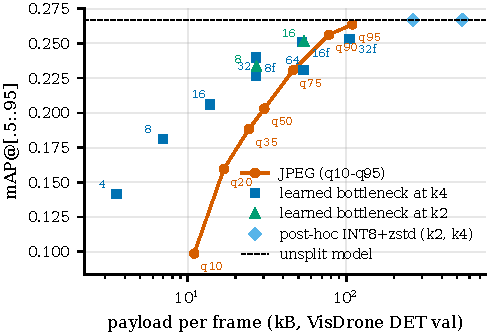
\includegraphics[width=\columnwidth]{learned_bottleneck.pdf}
\caption{Accuracy against payload on held-out VisDrone frames: JPEG at qualities 10--95, learned codes at two cuts
(labels: channels) and the post-hoc INT8+zstd splits.}
\label{fig:rate}
\end{figure}

\section{Model}\label{sec:model}
A camera at $F$ frames/s offers each frame to one option $c$: onboard inference, an image setting $q$ (JPEG quality,
video setting), or a split code $k$. Option $c$ has onboard time $e_c$, payload $b_c$ (bits), server time $s_c$ and
accuracy $A_c$ (mAP$_{50:95}$ on held-out VisDrone frames, our VisDrone-trained YOLOv8s). With goodput $B$ and one-way
delay $d$, it delivers $f_c(B) = F/\lceil F\max(e_c, b_c/B)\rceil$ frames/s. A frame is on time with probability
$p_c(B) = Q\big((R_c - B)/\sigma(B)\big)$, where $R_c = b_c/(D - e_c - d - s_c)$ is the rate the deadline $D = 300$~ms
needs, $Q$ the normal tail and $\sigma(B) \le sB$ the goodput spread. Its value is the accurate on-time rate
$U_c(B) = f_c(B)\,p_c(B)\,A_c$. Onboard times scale with the device's full-model time $t_{\mathrm{full}}$: a code that
runs a fraction $\phi_k$ of the detector's MACs onboard, plus encoder and quantiser work $\rho_k$, needs
$e_k = t_{\mathrm{full}}(\phi_k + \rho_k)$.

\section{The Break-Even Goodput}\label{sec:rule}
\begin{proposition}[Break-even goodput]\label{prop:be}
Let $m_k = \max(e_k, 1/F)$ for a code $k$, and fix $P<1$ with normal quantile $z_P$ and $z_P s < 1$. An image
setting $q$ with $P A_q \ge A_k$ and $e_q \le m_k$ gives $U_q(B) \ge U_k(B)$ whenever
$B \ge \max\big(b_q/m_k,\; R_q/(1 - z_P s)\big)$. Hence $k$ can beat every image setting only below
\begin{equation*}
B_{\mathrm{be}}(k) = \min_{q:\,P A_q \ge A_k,\; e_q \le m_k} \max\Big(\frac{b_q}{m_k},\; \frac{R_q}{1 - z_P s}\Big),
\end{equation*}
with $B_{\mathrm{be}} = \infty$ if no setting qualifies.
\end{proposition}
\begin{proof}
From $b_q \le B m_k$ and $e_q \le m_k$:
$\lceil F\max(e_q, b_q/B)\rceil \le \lceil F m_k\rceil = \max(1, \lceil F e_k\rceil) \le \lceil F\max(e_k, b_k/B)\rceil$,
so $f_q \ge f_k$. Since $\sigma(B) \le sB$, $B \ge R_q/(1 - z_P s)$ gives $p_q \ge P$. Hence
$U_q \ge P f_q A_q \ge f_k A_k \ge U_k$.
\end{proof}
\begin{corollary}[No coder raises the bound]\label{cor:coder}
$B_{\mathrm{be}}(k)$ depends on the code only through $A_k$ and $m_k$, not its payload $b_k$. It is non-decreasing in
$A_k$ and non-increasing in $m_k$. A better coder, even one at the task's rate--distortion limit, adds wins only below
$B_{\mathrm{be}}$.
\end{corollary}
\begin{proof}
$b_k$ does not appear in $B_{\mathrm{be}}(k)$. Raising $A_k$ shrinks the set of qualifying settings, so the minimum
cannot fall; raising $m_k$ lowers $b_q/m_k$ and enlarges the set, so it cannot rise.
\end{proof}
\begin{corollary}[Switching codes]\label{cor:switch}
A split that chooses among codes $k \in \mathcal K$ slot by slot can beat every image setting in a slot of goodput $B$
only if $B < \max_{k} B_{\mathrm{be}}(k)$.
\end{corollary}
\noindent Information-theoretic work bounds the rate a code needs for an accuracy and finds learned codes far from
it~\cite{shao2022taskoriented,tosc2026limits}. Corollary~\ref{cor:coder} is the system-level complement: closing that gap
shrinks $b_k$ but leaves $B_{\mathrm{be}}$ in place. A faster device shortens $m_k$ and raises the first term, until the
camera rate or the deadline term binds.

\textbf{Fading version.} Discounting both terms by the same low quantile of the goodput gives
$B_{\mathrm{be,f}}(k) = \min_P \min_{q} \max(b_q/m_k, R_q)/(1 - z_P s)$ with $s$ the link's measured relative spread. It
is an empirical rule; we test it below.

\textbf{Energy version.} With the radio's power $a + bB$, the image's encode energy $e_{\mathrm{enc}}$, the code's
onboard energy $e_c(k)$ and $S = b_{q^\ast} - b_k$ the bits saved against the matching setting $q^\ast$, the split uses
less energy per frame exactly when $B < B_E(k) = aS/(e_c(k) - e_{\mathrm{enc}} - bS)$.

\section{Tests}\label{sec:tests}
\textbf{Setup.} \BeCodes{} learned codes at the stride-4 and stride-8 cuts of the VisDrone YOLOv8s (frozen-detector
distillation, joint training of the server side, and a learned entropy model with a range coder), against
\BeJpegQualities{} JPEG qualities (every 5 from 10 to 95) on the same frames with the same detector, on
\BeMeasuredDevices{} measured devices (laptop GPU, Jetson Orin Nano, throttled Pi~5) and \BeSweepSpeeds{} swept speeds,
at goodputs in steps of \BeGridStepPct\,\%. Table~\ref{tab:tests} lists every test.

\begin{table*}[t]
\centering
\caption{Every test of the break-even goodput. Exceptions: model wins at or above $B_{\mathrm{be}}$ (or
$B_{\mathrm{be,f}}$ for fading links).}
\label{tab:tests}
\small
\begin{tabular}{@{}p{0.2\textwidth}p{0.6\textwidth}p{0.14\textwidth}@{}}
\toprule
Test & What it showed & Exceptions \\
\midrule
Model check & A code beats every JPEG setting in \BeCells{} cells; with only \BeJpegQualitiesCoarse{} qualities, in
\BeCellsCoarse{}: a coarse JPEG grid overstates the split. The largest winning goodput is a median \BeTightFastMedian\,\%
below $B_{\mathrm{be}}$ on the fast devices. & \BeViolations \\
Jointly trained codes & +\BeJointGainMin{} to +\BeJointGainMax{} mAP, significant for \BeJointPairedSig{} of
\BeJointPairedN{} codes; the smallest code's Pi $B_{\mathrm{be}}$ rises from \BePiBe{} to \BeJointPiBe~Mbit/s
(bootstrap 95\,\%: \BeCiJointPiLo--\BeCiJointPiHi) & \BeViolations \\
Detector tuned on JPEG & Split wins fall from \BeCells{} to \BeTunedCells{} cells; the smallest joint code's Pi
$B_{\mathrm{be}}$ falls to \BeTunedJointPiBe~Mbit/s & \BeTunedViolations \\
Learned entropy coder & \BeEcSaveZstdMin--\BeEcSaveZstdMax\,\% smaller than the zstd codes at equal accuracy, the same
$B_{\mathrm{be}}$ (\BeEcPairEcBe~Mbit/s on the Jetson for both), as Corollary~\ref{cor:coder} says & \BeEcViol \\
Low-delay video (x264/x265) & \VcSaveHtfUltra--\VcSaveHtfMedium\,\% fewer bytes than JPEG; the smallest joint code's
$B_{\mathrm{be}}$ falls from \VcJpegJointFastBe{} to \VcVideoJointFastBe~Mbit/s (Jetson); winning cells
\VcJpegWins{} $\to$ \VcBothWins & \VcBothExc \\
Inter-frame coded codes & \ViSaveMin--\ViSaveMax\,\% fewer code bytes; $B_{\mathrm{be}}$ unchanged, wins only added
below it (\ViBothWins{} cells) & \ViBothExc \\
Learned image codecs & \LicSaveMedian\,\% fewer bytes than JPEG, but encoders at \LicEncFracMin--\LicEncFracMax\,\% of
the detector's MACs: they never fit a code's frame time & \LicBothExc \\
Region-of-interest JPEG & Regions cover \VcRoiArea\,\% of the frame; median saving \VcSaveRoi\,\% at equal accuracy &
\VcBothExc \\
A second detector (YOLO11s) & $B_{\mathrm{be}}$ \SdPiBeMin--\SdPiBeMax~Mbit/s on the Pi, but no win: the onboard layers
take \SdPiOnboardMs{} of the \SdDeadlineMs~ms deadline & \SdExc \\
Fading links (simulator) & The constant bound fails for \BeSimModExcPct\,\% / \BeSimVehExcPct\,\% of simulated wins,
only on devices of $\le$\BeSimExcTfullMax~ms, by a median \BeSimModMargin\,\% / \BeSimVehMargin\,\%; the fading version
holds & \BeSimModFadingExc{} / \BeSimVehFadingExc \\
Measured mesh links (simulator) & Spread \BeSimMeshSpread; the constant bound fails for \BeSimMeshExcPct\,\% of wins; the
fading version holds & \BeSimMeshFadingExc \\
Energy (Pi constants) & A split saves energy only below \BeEnMax~kbit/s for any code; at 1~Mbit/s the smallest joint
code costs \BeEnJointRatio$\times$ its JPEG setting's energy & --- \\
\bottomrule
\end{tabular}
\end{table*}

\begin{figure}[t]
\centering
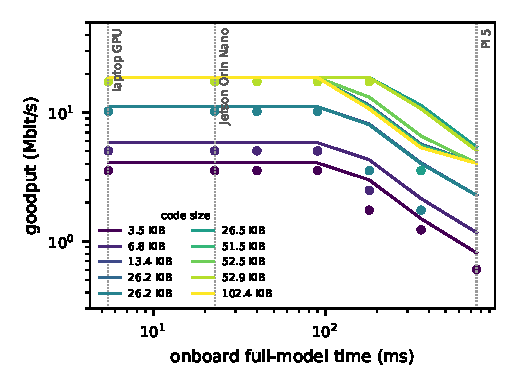
\includegraphics[width=\columnwidth]{break_even_map.pdf}
\caption{Break-even goodput of each learned code against the measured JPEG settings (lines, $P = \BePOn$) and the
largest goodput at which the model has the code beat all of them (dots), against the onboard full-model time.}
\label{fig:map}
\end{figure}

The check uses the model the proposition is derived in, so it confirms the derivation and its implementation, not
the model; the simulator and the boards test the model. Figure~\ref{fig:map} shows the bound and the largest winning
goodput of every code: on a Pi a code can win only below about 2~Mbit/s, on a fast device up to the camera rate.
Joint training raises $B_{\mathrm{be}}$ (better accuracy needs a better matching image), but part of its gain comes from
training only one side: with a detector tuned on JPEG the window narrows again. Stronger image codecs remove most of
the room a split had, which is Corollary~\ref{cor:coder} applied to the image side.

\section{On the Boards: Predicted, Then Measured}\label{sec:boards}
\textbf{The sweep.} A Raspberry Pi~5 camera sent to a Jetson Orin Nano over a batman-adv mesh. The codes and JPEG
were timed on each board (the codes take \BpCodeMsMin--\BpCodeMsMax~ms onboard on the Pi, JPEG \BpJpegOnb~ms), and the
link was serialised by netem at \BpRates~Mbit/s, every run started with the Pi below 60~$^\circ$C. The model,
from the board timings alone and committed before the sweep, predicted that no code beats JPEG at these goodputs,
because the code's onboard part caps it at about 4--5 frames/s. That held: the best option measured at every goodput
was a JPEG, no code exceeded \BpCodeFpsMax{} on-time results/s, and JPEG reached \BpJpegFpsEight{} at 8~Mbit/s. Cell
by cell, the model's on-time rate was a median \BpModelErrPct\,\% from the measured one over the \BpModelCellsBig{}
cells with at least one result per second ($r = \BpModelR$ over all \BpModelCells), and its best option was the
measured one at \BpModelBestMatch{} of \BpModelRates{} goodputs (at the other, both are JPEG). With a token-bucket link
instead, a low average goodput from a shared fast radio, the smallest code delivered \BpHtbCode{} on-time results/s at
0.5~Mbit/s against JPEG's \BpHtbJpeg: how the link is slow matters, which $t_{\mathrm{tx}} = b/B$ does not separate.

\textbf{CPU encoding on the Pi.} Scaling every onboard time by the full-model ratio (\BpScale{} on the throttled Pi)
is right for neural layers but not for CPU encoding: measured on the Pi, video encodes only \BpRatioMin--\BpRatioMax{}
times slower than on the host and JPEG \BpJpegRatio{} times. With every option at its measured Pi time, the smallest
joint code's $B_{\mathrm{be}}$ is \BpHeadJpegMeas~Mbit/s against JPEG (scaled: \BpHeadJpegRule) and
\BpHeadVideoMeas~Mbit/s with video (scaled: \BpHeadVideoRule); with video, no code has a winning cell on the Pi
(\BpWinsVideoMeas{} cells, \BpExc{} exceptions), as the sweep found. YOLO11s codes timed on the Pi are within
\BpYelevenDev\,\% of the scaled times.

\textbf{A fast camera.} The same benches timed the codes on a Jetson used as the camera: \BpJetCodeMsMin--\BpJetCodeMsMax~ms
onboard, while its CPU encodes JPEG \BpJetJpegRatio{} times slower than the host. On these measured times the smallest
joint code's $B_{\mathrm{be}}$ against JPEG is \BpJetHeadJpeg~Mbit/s, as scaled times give, and codes win in
\BpJetWinsJpeg{} cells: on a fast camera the rule predicts a real window. With video it is
\BpJetHeadVideoLo--\BpJetHeadVideoHi~Mbit/s, depending on the Jetson's video encode time, which we did not measure
(\BpJetExc{} exceptions). We did not sweep a Jetson camera live.

\section{Published Wins, Re-Read}\label{sec:published}
The rule says a split must be compared with the cheapest image of \emph{equal accuracy}. We re-read \BpLitPapers{}
published results with the numbers they report (Table~\ref{tab:published}). None of them makes that comparison.
Auto-Split's own ablation shows what it changes: its \BpLitAutoRaw$\times$ latency advantage over the raw image is
\BpLitAutoMatched$\times$ against its JPEG setting of equal mAP. Our own model shows the same effect on the image grid:
\BeCellsCoarse{} winning cells with \BeJpegQualitiesCoarse{} qualities against \BeCells{} with \BeJpegQualities. The
one result whose split path computes faster than its image path, before any transfer, wins everywhere, which the rule
allows ($B_{\mathrm{be}} = \infty$).
\begin{table*}[t]
\centering
\caption{Published split-computing results read against the break-even rule (numbers as each paper reports them).}
\label{tab:published}
\small
% Generated by evaluation/board_metrics_paper1.py from experiments/results/literature/published_splits.json
\begin{tabular}{@{}p{0.2\linewidth}p{0.2\linewidth}p{0.2\linewidth}p{0.32\linewidth}@{}}\toprule
Work & Setting & Image baseline & Read against the rule \\\midrule
Auto-Split~\cite{banitalebi2021autosplit} & YOLOv3, simulated edge & uncompressed image & 12.5$\times$ faster than raw; 1.9$\times$ against its own JPEG Q60 at equal mAP \\
Matsubara \& Levorato~\cite{matsubara2021neural} & Faster R-CNN, Jetson TX2 & JPEG at stored quality, unsplit detector & code at 0.355 mAP against an image at 0.370: not accuracy-matched \\
Matsubara \& Levorato~\cite{matsubara2020complex} & R-CNN, Pi~4 / TX2 & raw input tensor & no compressed image baseline \\
BottleFit~\cite{matsubara2022bottlefit} & classification, Jetson Nano & one JPEG quality & image not lowered to the code's accuracy \\
HECS-B~\cite{zhong2025hecsb} & classification, Jetson Nano & WebP, PNG & split path faster than the image path: no finite $B_{\mathrm{be}}$, wins everywhere \\
\bottomrule
\end{tabular}

\end{table*}

\section{Design Rule and Limitations}
\textbf{Design rule.} Before building a split, compute $B_{\mathrm{be}}$ from the code's accuracy and onboard time, the
image codec's rate--accuracy curve on the same frames (with the best detector the server can run for it) and the
device's measured onboard times. If the link's goodput is mostly above $B_{\mathrm{be}}$, send the image; on a fading
link use $B_{\mathrm{be,f}}$ with the measured spread.

\textbf{Limitations.} One onboard computer was swept live (a fanless Pi~5); a Jetson was timed as a camera, not swept,
and its video encode time was not measured. The live link was a netem-serialised rate limit; a shared fast radio can
favour a small code. All accuracies are for VisDrone with YOLOv8s and YOLO11s. The fading version is empirical. The MPEG
feature-coding standard was not run: its reference software is hosted for MPEG members, and the open CompressAI-Vision
pipelines need the VVC reference codec and other detector families; Corollary~\ref{cor:coder} bounds what any feature
coder could add.

\section{Conclusion}
A learned split code pays off only below a goodput that its accuracy, the device's onboard time and the image codec's
rate curve fix in advance, and that no coder can raise. In \BeCells{} model cells and every stress test the rule had
no exception where it is proved, and its fading version none where it is empirical. On real boards its prediction held
before it was measured: on a Pi~5 camera JPEG wins at every goodput, and with low-delay video a split never wins; on a
fast camera, a window below a few Mbit/s remains. Published wins measured against weaker image baselines overstate
that window.

\bibliographystyle{IEEEtran}
\bibliography{references}
\end{document}
